\documentclass[12pt,a4paper]{article}
\usepackage[utf8]{inputenc}
\usepackage[margin=1in]{geometry}
\usepackage{graphicx}
\usepackage{hyperref}
\usepackage{listings}
\usepackage{xcolor}
\usepackage{float}
\usepackage{booktabs}
\usepackage{tikz}
\usetikzlibrary{positioning}
\usepackage{caption}
\usepackage{subcaption}
\usepackage{amsmath}
\usepackage{algorithm}
\usepackage{algpseudocode}

% Code listing configuration
\lstset{
    basicstyle=\ttfamily\small,
    breaklines=true,
    frame=single,
    language=Python,
    showstringspaces=false,
    commentstyle=\color{green!60!black},
    keywordstyle=\color{blue},
    stringstyle=\color{red},
}

% Hyperref configuration
\hypersetup{
    colorlinks=true,
    linkcolor=blue,
    filecolor=magenta,
    urlcolor=cyan,
    citecolor=green,
}

\begin{document}

% ===========================
% TITLE PAGE
% ===========================
\begin{titlepage}
    \centering
    \vspace*{2cm}

    {\Huge\bfseries JobSync: Intelligent Job Search Management Platform\par}
    \vspace{1cm}
    {\Large\bfseries With AI-Powered Resume Analysis and Course Recommendations\par}
    \vspace{2cm}

    {\large Computer Science and Engineering\par}
    \vspace{1.5cm}

    {\large\textbf{Project Report}\par}
    {\large Academic Year 2024-2025\par}
    \vspace{1cm}

    {\large\today\par}

    \vfill
\end{titlepage}

% ===========================
% ABSTRACT
% ===========================
\newpage
\section*{Abstract}
\addcontentsline{toc}{section}{Abstract}

In today's competitive job market, job seekers face significant challenges in managing multiple applications, tracking their progress, and identifying skill gaps for desired positions. JobSync addresses these challenges by providing an intelligent, self-hosted web platform that combines job application tracking with AI-powered resume analysis and personalized course recommendations.

This project implements a full-stack distributed system utilizing modern technologies including Next.js 15, Python FastAPI microservices, machine learning models for natural language processing, and cloud deployment infrastructure. The system employs sentence transformers for semantic skill matching, spaCy for information extraction, and LangChain with OpenAI GPT models for intelligent resume analysis.

Key features include real-time job application tracking, AI-powered resume review, automated skill gap analysis, personalized course recommendations from 585+ Coursera courses, and comprehensive activity monitoring. The platform is deployed on Google Cloud Platform using Docker containerization, demonstrating enterprise-grade scalability and reliability.

The project successfully integrates concepts from multiple computer science domains: Machine Learning (NLP, embeddings), Distributed Systems (microservices architecture), Database Management (relational modeling with Prisma ORM), Cloud Computing (GCP deployment), Network Administration (Docker networking, REST APIs), Algorithm Engineering (cosine similarity, fuzzy matching), Software Security (authentication, API key management), Data Mining (skill extraction, pattern matching), Operating Systems (Linux containers), and Artificial Intelligence (LLM integration, semantic search).

% ===========================
% TABLE OF CONTENTS
% ===========================
\newpage
\tableofcontents
\newpage

% ===========================
% INTRODUCTION
% ===========================
\section{Introduction}

\subsection{Background}

The modern job search process has become increasingly complex, requiring job seekers to manage multiple applications across various platforms, maintain updated resumes, and continuously acquire new skills to remain competitive. Traditional job search tools often lack integration between application tracking, skill assessment, and learning resources, forcing users to rely on disconnected systems.

The rise of artificial intelligence and machine learning has created opportunities to automate many aspects of career development, from resume optimization to personalized learning path generation. However, most existing solutions are either proprietary cloud services that don't respect user data privacy, or lack the sophisticated AI capabilities needed for meaningful insights.

JobSync was conceived as a comprehensive, open-source solution that gives users complete control over their job search data while leveraging state-of-the-art AI technologies. The platform addresses the fragmentation in job search tools by providing an integrated ecosystem for tracking, analysis, and skill development.

\subsection{Problem Statement}

Job seekers encounter several critical challenges in their career development journey:

\begin{enumerate}
    \item \textbf{Application Management Complexity}: Tracking dozens or hundreds of applications across multiple platforms becomes overwhelming without a centralized system. Users lose track of application statuses, deadlines, and follow-up requirements.

    \item \textbf{Skill Gap Identification}: Understanding which skills are required for desired positions and which skills need to be acquired is time-consuming and often inaccurate when done manually.

    \item \textbf{Resume Optimization}: Creating tailored resumes for different positions requires understanding how well one's experience matches job requirements, which is difficult to assess objectively.

    \item \textbf{Learning Path Confusion}: Even after identifying skill gaps, finding relevant, high-quality courses from thousands of options is challenging and time-intensive.

    \item \textbf{Data Privacy Concerns}: Most existing job search platforms store user data on proprietary servers, raising privacy and data ownership concerns.

    \item \textbf{Lack of Analytics}: Users have limited visibility into their job search patterns, success rates, and areas for improvement.
\end{enumerate}

These problems result in inefficient job searches, missed opportunities, and prolonged unemployment periods, particularly affecting early-career professionals who lack established networks and experience in job hunting strategies.

\subsection{Purpose of the Project}

JobSync aims to solve these challenges by providing a comprehensive, AI-powered, self-hosted job search management platform with the following objectives:

\begin{itemize}
    \item Centralize job application tracking with detailed status management and deadline reminders
    \item Leverage natural language processing and machine learning to extract skills from resumes and job descriptions automatically
    \item Provide AI-powered resume analysis using large language models (OpenAI GPT) to offer personalized improvement suggestions
    \item Implement semantic search algorithms to match job seekers with the most relevant learning resources
    \item Enable complete data privacy through self-hosted deployment using Docker containers
    \item Offer comprehensive analytics dashboards showing job search progress and patterns
    \item Create a scalable microservices architecture that can be extended with additional features
    \item Demonstrate practical applications of multiple computer science concepts in a real-world system
\end{itemize}

% ===========================
% OBJECTIVES
% ===========================
\section{Objectives}

The primary objectives of this project are:

\begin{enumerate}
    \item \textbf{Develop a Full-Stack Job Management Platform}
    \begin{itemize}
        \item Implement a responsive web interface using React and Next.js 15
        \item Design and implement a relational database schema using SQLite and Prisma ORM
        \item Create RESTful APIs for all application features
        \item Implement secure user authentication and authorization using NextAuth.js
    \end{itemize}

    \item \textbf{Implement Machine Learning-Based Skill Extraction}
    \begin{itemize}
        \item Develop an NLP pipeline using spaCy for extracting technical skills from unstructured text
        \item Implement phrase matching algorithms to identify 150+ technical skills
        \item Apply fuzzy string matching for handling skill variations and synonyms
        \item Create a skill comparison engine for matching resumes against job requirements
    \end{itemize}

    \item \textbf{Build an AI-Powered Resume Analysis System}
    \begin{itemize}
        \item Integrate OpenAI GPT models using LangChain framework
        \item Design prompts for generating actionable resume improvement suggestions
        \item Implement streaming responses for real-time feedback
        \item Calculate job-resume match scores using AI-driven analysis
    \end{itemize}

    \item \textbf{Create a Course Recommendation Engine}
    \begin{itemize}
        \item Implement sentence transformers (all-MiniLM-L6-v2) for generating semantic embeddings
        \item Develop a cosine similarity algorithm for matching skills to courses
        \item Build a database of 585+ Coursera courses with pre-computed embeddings
        \item Implement semantic search functionality for course discovery
    \end{itemize}

    \item \textbf{Design a Microservices Architecture}
    \begin{itemize}
        \item Separate concerns into frontend (Next.js) and ML backend (FastAPI) services
        \item Implement inter-service communication using HTTP REST APIs
        \item Design for horizontal scalability and fault tolerance
        \item Apply containerization using Docker for consistent deployment
    \end{itemize}

    \item \textbf{Deploy on Cloud Infrastructure}
    \begin{itemize}
        \item Configure Google Cloud Platform compute instances
        \item Implement Docker Compose orchestration for multi-container deployment
        \item Set up networking and security configurations
        \item Implement CI/CD considerations for automated deployments
    \end{itemize}

    \item \textbf{Demonstrate CS Domain Integration}
    \begin{itemize}
        \item Apply machine learning algorithms (NLP, embeddings, cosine similarity)
        \item Implement distributed systems concepts (microservices, service discovery)
        \item Design and optimize database schemas (normalization, indexing)
        \item Apply algorithm engineering (fuzzy matching, similarity search)
        \item Implement software security measures (authentication, API security)
        \item Demonstrate cloud computing deployment (containerization, orchestration)
        \item Apply data mining techniques (pattern matching, information extraction)
        \item Utilize operating system features (process management, networking)
        \item Implement AI systems (LLM integration, prompt engineering)
        \item Configure network administration (TCP/IP, Docker networking, CORS)
    \end{itemize}
\end{enumerate}

% ===========================
% SYSTEM REQUIREMENTS
% ===========================
\section{System Requirements}

\subsection{Hardware Requirements}

\subsubsection{Development Environment}
\begin{itemize}
    \item \textbf{Processor}: Intel Core i5 or equivalent (recommended: i7 or Apple M1/M2)
    \item \textbf{RAM}: Minimum 8GB (recommended: 16GB for running ML models)
    \item \textbf{Storage}: 20GB free disk space for Docker images, models, and databases
    \item \textbf{Network}: Broadband internet connection for API calls to OpenAI services
\end{itemize}

\subsubsection{Production/Cloud Deployment}
\begin{itemize}
    \item \textbf{VM Instance}: GCP e2-medium or equivalent (2 vCPUs, 4GB RAM)
    \item \textbf{Storage}: 30GB persistent SSD for application and data storage
    \item \textbf{Network}: Static external IP address for public access
    \item \textbf{Load Considerations}: ML service requires approximately 2GB RAM for model loading
\end{itemize}

\subsection{Software Requirements}

\subsubsection{Core Technologies}
\begin{itemize}
    \item \textbf{Operating System}: Linux (Ubuntu 22.04 LTS recommended), macOS, or Windows with WSL2
    \item \textbf{Docker}: Version 24.0 or higher with Docker Compose v2
    \item \textbf{Node.js}: Version 18.x or higher for Next.js application
    \item \textbf{Python}: Version 3.11 for ML microservice
    \item \textbf{Web Browser}: Modern browser with JavaScript support (Chrome, Firefox, Safari, Edge)
\end{itemize}

\subsubsection{Frontend Stack}
\begin{itemize}
    \item \textbf{Framework}: Next.js 15.5.7 (React 19.0)
    \item \textbf{UI Library}: shadcn/ui components with Radix UI primitives
    \item \textbf{Styling}: Tailwind CSS 3.4
    \item \textbf{State Management}: React Hooks (useState, useEffect, useContext)
    \item \textbf{Form Handling}: React Hook Form with Zod validation
    \item \textbf{Charts}: Nivo for data visualization
    \item \textbf{Rich Text}: Tiptap editor for resume and job description editing
\end{itemize}

\subsubsection{Backend Stack}
\begin{itemize}
    \item \textbf{Database}: SQLite 3 with Prisma ORM 6.19
    \item \textbf{Authentication}: NextAuth.js 5.0 with credential-based auth
    \item \textbf{API Framework}: Next.js App Router API routes
    \item \textbf{ML Framework}: FastAPI 0.100+ for Python microservice
\end{itemize}

\subsubsection{Machine Learning Libraries}
\begin{itemize}
    \item \textbf{NLP}: spaCy 3.7 with en\_core\_web\_md model
    \item \textbf{Embeddings}: sentence-transformers (all-MiniLM-L6-v2 model)
    \item \textbf{LLM Integration}: LangChain 0.2.9 with OpenAI integration
    \item \textbf{AI Models}: OpenAI GPT-3.5-turbo for resume analysis
    \item \textbf{ML Utilities}: scikit-learn for cosine similarity, numpy, pandas
    \item \textbf{Text Processing}: PyPDF2 for PDF parsing, rapidfuzz for fuzzy matching
\end{itemize}

\subsubsection{Cloud and DevOps}
\begin{itemize}
    \item \textbf{Cloud Platform}: Google Cloud Platform (Compute Engine)
    \item \textbf{Container Registry}: Docker Hub for image distribution
    \item \textbf{Orchestration}: Docker Compose for multi-container management
    \item \textbf{Monitoring}: Docker logs, GCP monitoring
    \item \textbf{Networking}: Docker bridge networks, reverse proxy considerations
\end{itemize}

\subsubsection{Development Tools}
\begin{itemize}
    \item \textbf{Version Control}: Git with GitHub hosting
    \item \textbf{Package Managers}: npm for Node.js, pip for Python
    \item \textbf{Testing}: Jest for unit tests, Playwright for E2E testing
    \item \textbf{Linting}: ESLint for code quality, Prettier for formatting
    \item \textbf{Database Tools}: Prisma Studio for database visualization
\end{itemize}

\subsubsection{External Services}
\begin{itemize}
    \item \textbf{OpenAI API}: Valid API key with GPT-3.5-turbo access
    \item \textbf{Coursera Data}: Pre-downloaded dataset with 585 courses
    \item \textbf{Domain/SSL}: Optional for production deployment
\end{itemize}

% ===========================
% EXISTING SYSTEM
% ===========================
\section{Existing System}

\subsection{Analysis of Current Job Search Tools}

Several platforms exist in the job search management space, each with distinct characteristics and limitations:

\subsubsection{LinkedIn Job Tracker}
\textbf{Features}:
\begin{itemize}
    \item Integrated with LinkedIn's professional network
    \item Basic application status tracking
    \item Job recommendations based on profile
\end{itemize}

\textbf{Limitations}:
\begin{itemize}
    \item Limited to LinkedIn ecosystem only
    \item No AI-powered resume analysis
    \item No personalized learning recommendations
    \item Data privacy concerns with proprietary cloud storage
    \item No skill gap analysis features
\end{itemize}

\subsubsection{Huntr}
\textbf{Features}:
\begin{itemize}
    \item Visual Kanban board for application tracking
    \item Chrome extension for job import
    \item Basic activity tracking
\end{itemize}

\textbf{Limitations}:
\begin{itemize}
    \item Subscription-based pricing model
    \item No ML-based skill extraction
    \item Limited customization options
    \item Cloud-only deployment (no self-hosting)
    \item No integrated course recommendations
\end{itemize}

\subsubsection{Teal}
\textbf{Features}:
\begin{itemize}
    \item Resume builder with templates
    \item Job application tracking
    \item Basic resume analysis
\end{itemize}

\textbf{Limitations}:
\begin{itemize}
    \item Freemium model with feature restrictions
    \item Generic resume suggestions without AI personalization
    \item No skill-to-course matching system
    \item Closed-source proprietary software
    \item Limited API access for integrations
\end{itemize}

\subsection{General Limitations of Existing Systems}

\begin{enumerate}
    \item \textbf{Lack of AI-Powered Analysis}: Most systems provide basic tracking without intelligent analysis of resumes or job matches using modern LLMs.

    \item \textbf{No Personalized Learning Integration}: Existing platforms don't connect skill gaps with specific learning resources, forcing users to manually search for courses.

    \item \textbf{Privacy and Data Ownership}: Cloud-based systems store sensitive career data on external servers, with unclear data retention and usage policies.

    \item \textbf{Limited Customization}: Proprietary platforms don't allow customization of features, workflows, or data models to individual needs.

    \item \textbf{No Self-Hosting Options}: Most solutions require subscription to cloud services, preventing organizations from hosting internally.

    \item \textbf{Inadequate Skill Matching}: Simple keyword matching fails to understand semantic relationships between skills and job requirements.

    \item \textbf{Fragmented Workflow}: Users must switch between multiple tools for tracking, analysis, and learning, disrupting workflow efficiency.

    \item \textbf{Cost Barriers}: Premium features often require expensive subscriptions, limiting access for students and early-career professionals.

    \item \textbf{Vendor Lock-in}: Proprietary formats and lack of export capabilities create dependency on specific platforms.

    \item \textbf{Limited ML Capabilities}: Existing tools don't leverage state-of-the-art NLP models like transformers and embeddings for semantic understanding.
\end{enumerate}

\subsection{Justification for New System}

JobSync addresses these limitations by providing:
\begin{itemize}
    \item Open-source codebase allowing full customization and transparency
    \item Self-hosted deployment giving users complete data control
    \item State-of-the-art AI integration using GPT models and sentence transformers
    \item Seamless integration between tracking, analysis, and learning recommendations
    \item Advanced NLP for accurate skill extraction and semantic matching
    \item Cost-effective solution with no subscription requirements
    \item Microservices architecture for scalability and maintainability
    \item Comprehensive analytics for data-driven job search optimization
\end{itemize}

% ===========================
% PROPOSED SYSTEM
% ===========================
\section{Proposed System}

\subsection{Description of Solution}

JobSync is a comprehensive, AI-powered job search management platform designed as a distributed system with three primary layers:

\begin{enumerate}
    \item \textbf{Presentation Layer}: A modern, responsive web interface built with Next.js 15 and React 19, providing intuitive user experiences for job tracking, resume management, and skill analysis.

    \item \textbf{Application Layer}: Next.js API routes handling business logic, database operations, user authentication, and orchestration of ML services.

    \item \textbf{ML Services Layer}: A Python FastAPI microservice providing NLP-based skill extraction, semantic course recommendations, and integration with OpenAI LLMs.
\end{enumerate}

\subsubsection{Core Capabilities}

\textbf{1. Job Application Management}
\begin{itemize}
    \item Track unlimited job applications with customizable statuses
    \item Store complete job details: company, position, location, salary range, deadlines
    \item Link applications to specific resumes for version tracking
    \item Manage interview schedules and contact information
    \item Filter and search applications by multiple criteria
\end{itemize}

\textbf{2. AI-Powered Resume Analysis}
\begin{itemize}
    \item Upload resumes in PDF format with automatic text extraction
    \item Generate comprehensive resume reviews using GPT-3.5-turbo
    \item Receive personalized suggestions for improvement
    \item Compare resume against specific job descriptions
    \item Calculate match scores based on skill alignment
\end{itemize}

\textbf{3. Intelligent Skill Gap Analysis}
\begin{itemize}
    \item Automatic extraction of 150+ technical skills from resumes
    \item NLP-based parsing of job requirement skills
    \item Semantic comparison using fuzzy matching algorithms
    \item Visual representation of matched vs. missing skills
    \item Percentage-based match scoring
\end{itemize}

\textbf{4. Personalized Course Recommendations}
\begin{itemize}
    \item Semantic search across 585 Coursera courses
    \item Recommendations based on skill gaps using sentence transformers
    \item Ranking courses by relevance using cosine similarity
    \item Display course metadata: provider, rating, duration, skills gained
    \item Direct enrollment links to course platforms
\end{itemize}

\textbf{5. Activity Tracking and Analytics}
\begin{itemize}
    \item Time tracking for job search activities
    \item Categorization by activity types (networking, applying, interviewing)
    \item Visual dashboards showing application trends
    \item Calendar heatmaps for activity patterns
    \item Success rate analytics
\end{itemize}

\subsection{Architecture Diagram}

\begin{figure}[H]
\centering
\includegraphics[width=\textwidth]{arch.png}
\caption{JobSync System Architecture - Complete 6-Layer Design with ML Service Components}
\label{fig:architecture}
\end{figure}

The architecture follows a layered microservices design:

\textbf{Layer 1 - User Layer}: Web browsers (Chrome, Firefox, Safari, Edge) supporting HTML5, CSS3, and JavaScript ES6+ communicate via HTTP/HTTPS requests.

\textbf{Layer 2 - Frontend Layer}: Next.js 15 with React 19 provides server-side rendering (SSR) using the App Router. The UI is built with Tailwind CSS and shadcn/ui components for a modern, responsive experience.

\textbf{Layer 3 - API Gateway Layer}: Next.js API Routes in the App Router handle RESTful APIs, request validation, and error handling, orchestrating service communication.

\textbf{Layer 4 - Backend Services Layer}: A microservices architecture includes:
\begin{itemize}
    \item \textbf{Auth Service}: NextAuth.js with JWT sessions, bcrypt password hashing, and OAuth support
    \item \textbf{Database Service}: SQLite with Prisma ORM for type-safe queries and migration management
    \item \textbf{Business Logic}: Server Actions for job management and resume processing
\end{itemize}

\textbf{Layer 5 - ML Service Layer}: FastAPI (Python 3.11) on port 8000 provides four core ML components:
\begin{itemize}
    \item \textbf{Skill Extractor}: Uses spaCy (en\_core\_web\_md), PhraseMatcher algorithm, and RapidFuzz fuzzy matching against 150+ technical skills
    \item \textbf{Course Recommender}: Employs Sentence Transformers (all-MiniLM-L6-v2 model) with cosine similarity across 585 Coursera courses
    \item \textbf{Skill Comparator}: Analyzes resume vs job descriptions, calculates match percentages, identifies skill gaps using semantic understanding
    \item \textbf{Data Storage}: Manages pre-computed embeddings with Pickle serialization for fast vector search and embedding cache
\end{itemize}

\textbf{Layer 6 - External Services}: Integration with OpenAI GPT-3.5-turbo for resume review and job match scoring, Coursera course database with 585 courses and metadata, and Google Cloud Platform (GCP) Compute Engine e2-medium instance in asia-south1-a for hosting.

\subsection{Data Flow Diagram}

\subsubsection{Level 0 DFD (Context Diagram)}

\begin{figure}[H]
\centering
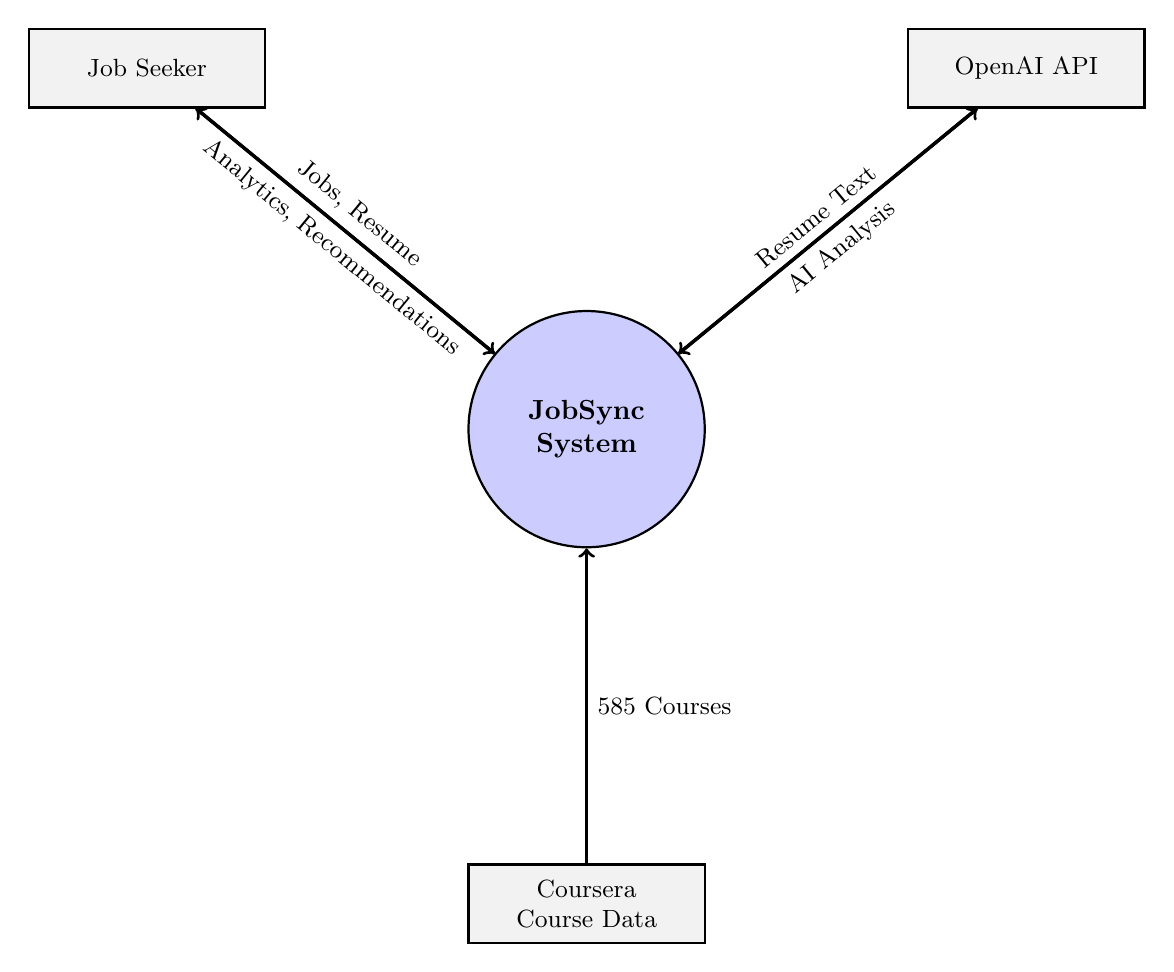
\begin{tikzpicture}[
    node distance=4cm,
    process/.style={circle, draw, thick, minimum size=3cm, align=center, fill=blue!20, font=\bfseries},
    entity/.style={rectangle, draw, thick, minimum width=3cm, minimum height=1cm, align=center, fill=gray!10, font=\small},
    arrow/.style={->, very thick}
]

% Central Process
\node[process] (system) {JobSync\\System};

% External Entities
\node[entity, above left=3cm and 3cm of system] (user) {Job Seeker};
\node[entity, above right=3cm and 3cm of system] (openai) {OpenAI API};
\node[entity, below=of system] (courses) {Coursera\\Course Data};

% Data Flows with labels
\draw[arrow] (user) -- node[above, sloped, font=\small] {Jobs, Resume} (system);
\draw[arrow] (system) -- node[below, sloped, font=\small] {Analytics, Recommendations} (user);
\draw[arrow] (system) -- node[above, sloped, font=\small] {Resume Text} (openai);
\draw[arrow] (openai) -- node[below, sloped, font=\small] {AI Analysis} (system);
\draw[arrow] (courses) -- node[right, font=\small] {585 Courses} (system);

\end{tikzpicture}
\caption{Level 0 Data Flow Diagram - System Context}
\label{fig:dfd0}
\end{figure}

\subsubsection{Level 1 DFD (Major Processes)}

\begin{figure}[H]
\centering
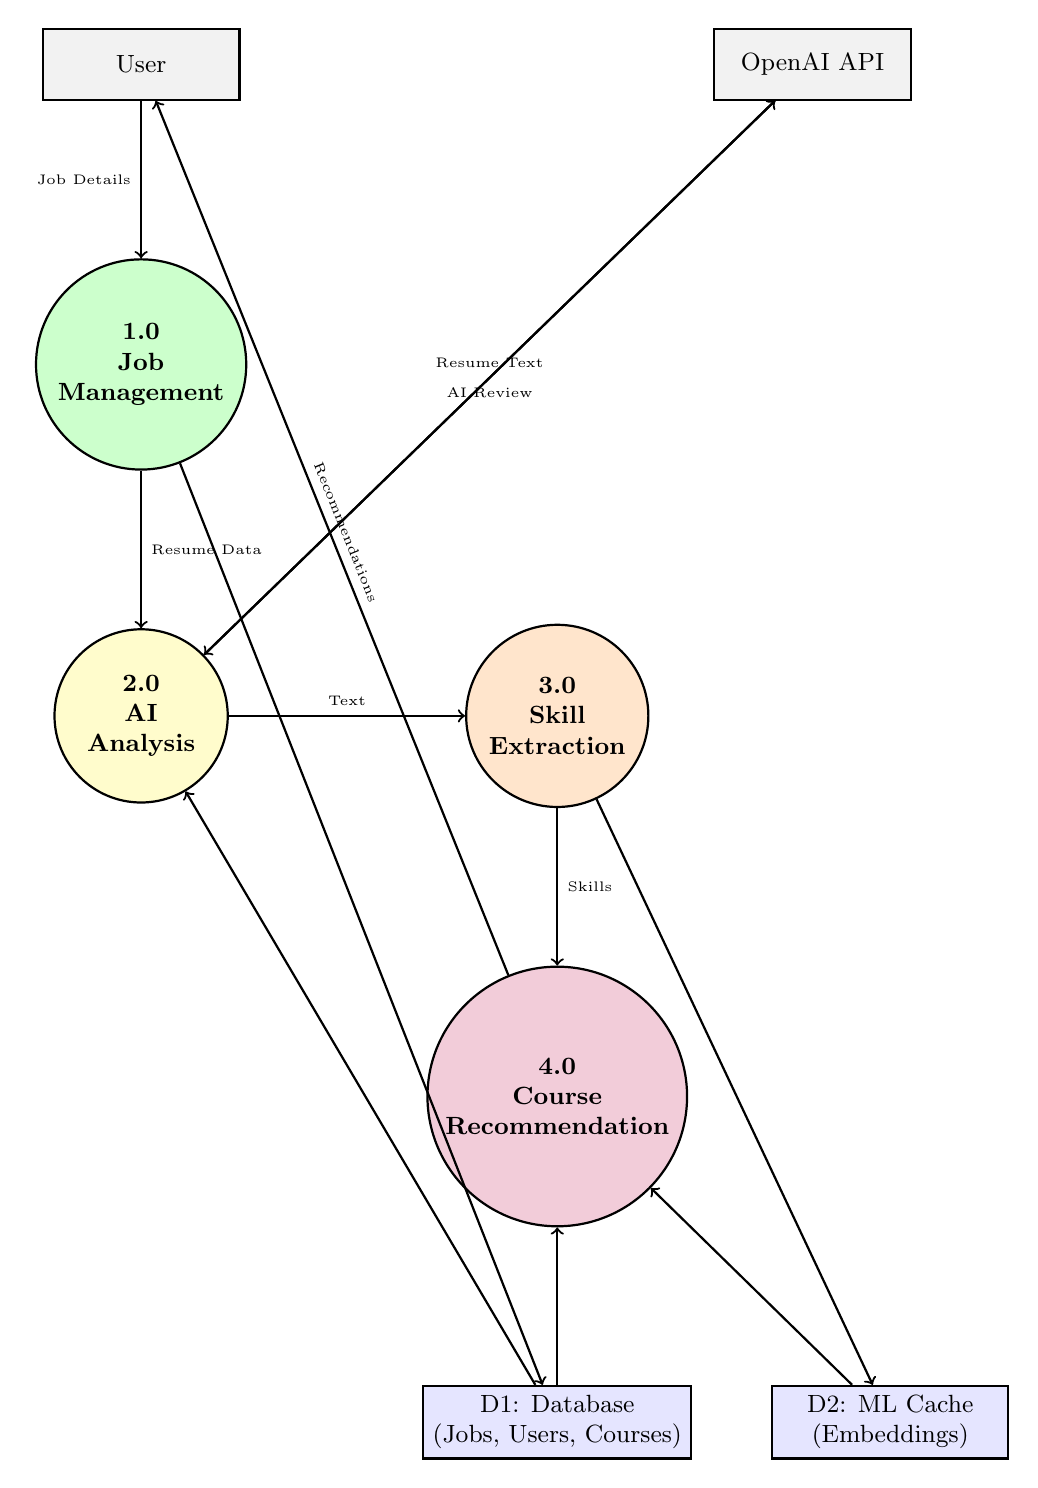
\begin{tikzpicture}[
    node distance=3cm,
    process/.style={circle, draw, thick, minimum size=2.2cm, align=center, font=\small\bfseries, fill=green!20},
    entity/.style={rectangle, draw, thick, minimum width=2.5cm, minimum height=0.9cm, align=center, font=\small, fill=gray!10},
    datastore/.style={rectangle, draw, thick, minimum width=3cm, minimum height=0.8cm, align=center, font=\small, fill=blue!10},
    arrow/.style={->, thick}
]

% External entities
\node[entity] (user) {User};
\node[entity, right=6cm of user] (openai) {OpenAI API};

% Processes
\node[process, below=2cm of user] (p1) {1.0\\Job\\Management};
\node[process, below=2cm of p1, fill=yellow!20] (p2) {2.0\\AI\\Analysis};
\node[process, right=3cm of p2, fill=orange!20] (p3) {3.0\\Skill\\Extraction};
\node[process, below=2cm of p3, fill=purple!20] (p4) {4.0\\Course\\Recommendation};

% Data Stores
\node[datastore, below=2cm of p4] (db) {D1: Database\\(Jobs, Users, Courses)};
\node[datastore, right=1cm of db] (cache) {D2: ML Cache\\(Embeddings)};

% Flows
\draw[arrow] (user) -- node[left, font=\tiny] {Job Details} (p1);
\draw[arrow] (p1) -- node[right, font=\tiny] {Resume Data} (p2);
\draw[arrow] (p2) -- node[above, font=\tiny] {Resume Text} (openai);
\draw[arrow] (openai) -- node[below, font=\tiny] {AI Review} (p2);
\draw[arrow] (p2) -- node[above, font=\tiny] {Text} (p3);
\draw[arrow] (p3) -- node[right, font=\tiny] {Skills} (p4);
\draw[arrow] (p4) -- node[above, sloped, font=\tiny] {Recommendations} (user);
\draw[arrow] (p1) -- (db);
\draw[arrow] (db) -- (p2);
\draw[arrow] (db) -- (p4);
\draw[arrow] (p3) -- (cache);
\draw[arrow] (cache) -- (p4);

\end{tikzpicture}
\caption{Level 1 DFD - Major Processes: Job Management, AI Analysis, Skill Extraction, Course Recommendation}
\label{fig:dfd1}
\end{figure}

\subsection{ER Diagram / Database Schema}

\begin{figure}[H]
\centering
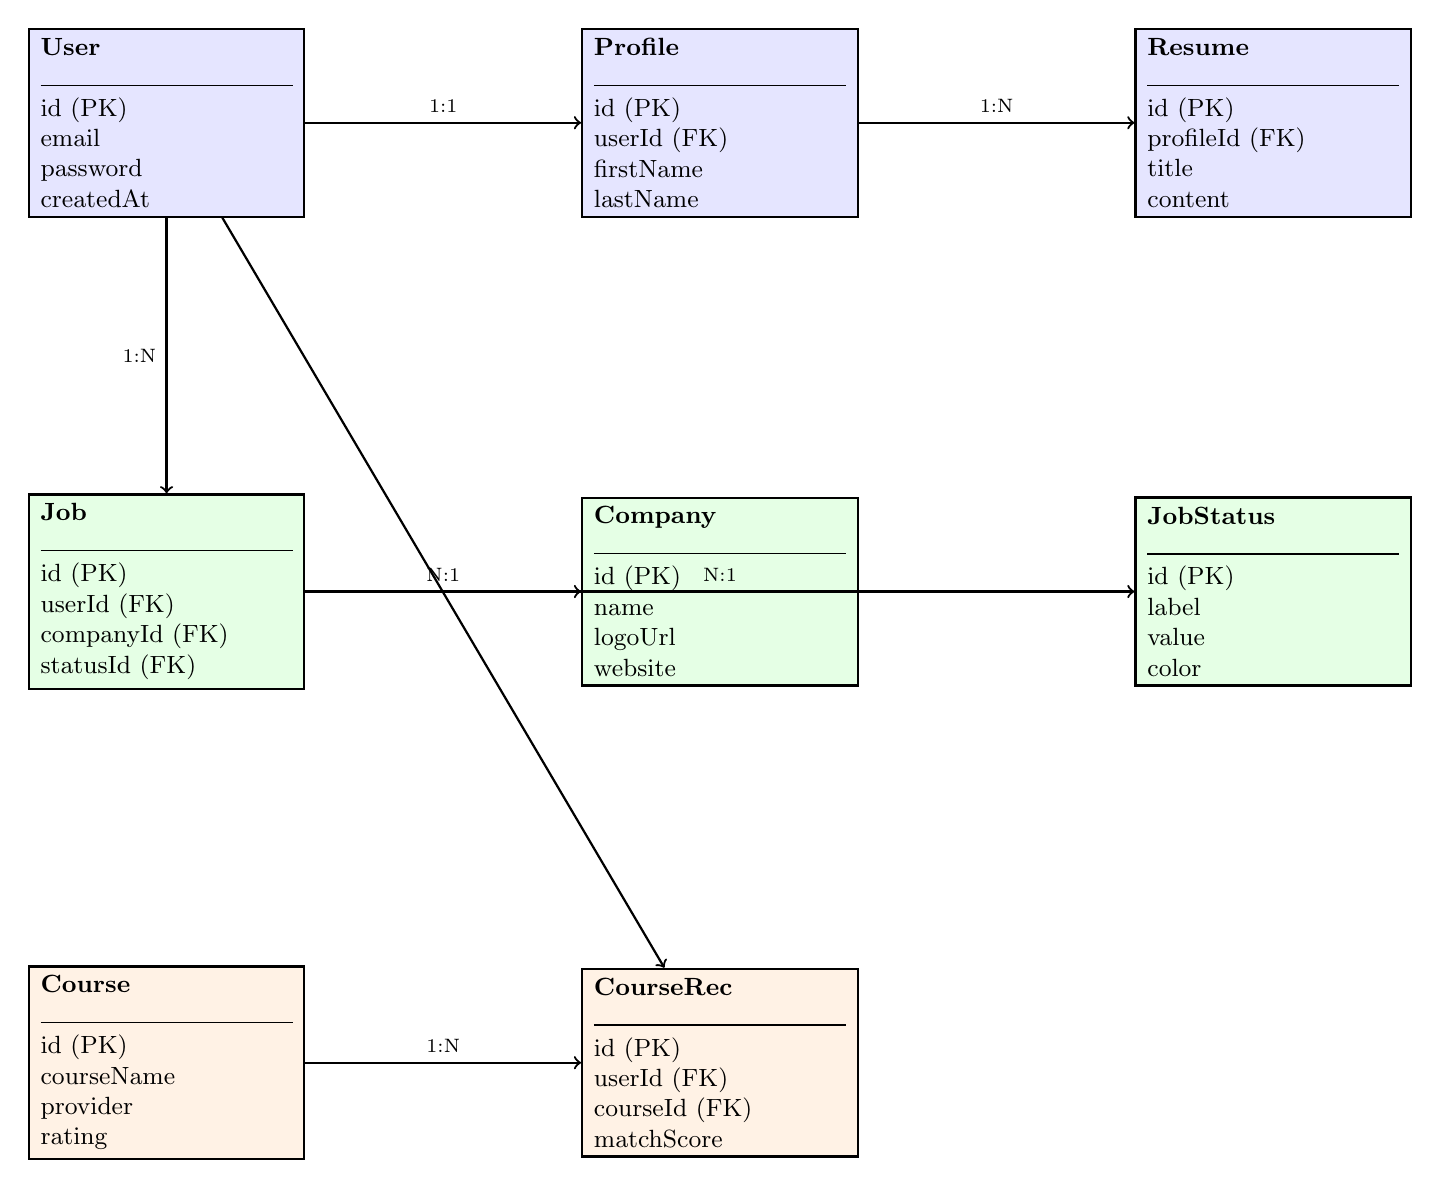
\begin{tikzpicture}[
    node distance=3.5cm,
    entity/.style={rectangle, draw, thick, minimum width=3.5cm, minimum height=2cm, align=left, fill=blue!10, font=\small},
    arrow/.style={->, thick}
]

% Top row - User entities
\node[entity] (user) {\textbf{User}\\
\rule{3.2cm}{0.4pt}\\
id (PK)\\
email\\
password\\
createdAt};

\node[entity, right=of user] (profile) {\textbf{Profile}\\
\rule{3.2cm}{0.4pt}\\
id (PK)\\
userId (FK)\\
firstName\\
lastName};

\node[entity, right=of profile] (resume) {\textbf{Resume}\\
\rule{3.2cm}{0.4pt}\\
id (PK)\\
profileId (FK)\\
title\\
content};

% Middle row - Job entities
\node[entity, below=of user, fill=green!10] (job) {\textbf{Job}\\
\rule{3.2cm}{0.4pt}\\
id (PK)\\
userId (FK)\\
companyId (FK)\\
statusId (FK)};

\node[entity, right=of job, fill=green!10] (company) {\textbf{Company}\\
\rule{3.2cm}{0.4pt}\\
id (PK)\\
name\\
logoUrl\\
website};

\node[entity, right=of company, fill=green!10] (status) {\textbf{JobStatus}\\
\rule{3.2cm}{0.4pt}\\
id (PK)\\
label\\
value\\
color};

% Bottom row - Course entities
\node[entity, below=of job, fill=orange!10] (course) {\textbf{Course}\\
\rule{3.2cm}{0.4pt}\\
id (PK)\\
courseName\\
provider\\
rating};

\node[entity, right=of course, fill=orange!10] (recommend) {\textbf{CourseRec}\\
\rule{3.2cm}{0.4pt}\\
id (PK)\\
userId (FK)\\
courseId (FK)\\
matchScore};

% Relationships with cardinality
\draw[arrow] (user) -- node[above, font=\scriptsize] {1:1} (profile);
\draw[arrow] (profile) -- node[above, font=\scriptsize] {1:N} (resume);
\draw[arrow] (user) -- node[left, font=\scriptsize] {1:N} (job);
\draw[arrow] (job) -- node[above, font=\scriptsize] {N:1} (company);
\draw[arrow] (job) -- node[above, font=\scriptsize] {N:1} (status);
\draw[arrow] (course) -- node[above, font=\scriptsize] {1:N} (recommend);
\draw[arrow] (user) -- (recommend);

\end{tikzpicture}
\caption{Entity Relationship Diagram - Core Database Entities with Primary Keys (PK) and Foreign Keys (FK)}
\label{fig:er}
\end{figure}

\subsubsection{Key Database Tables}

\textbf{1. User Table}
\begin{itemize}
    \item Stores user authentication credentials
    \item One-to-many relationships with Profile, Job, Activity
    \item Encrypted password storage using bcrypt
\end{itemize}

\textbf{2. Resume Table}
\begin{itemize}
    \item Stores resume metadata and content
    \item Foreign key to Profile
    \item Sections include: ContactInfo, WorkExperience, Education, Skills
    \item Supports multiple resumes per profile
\end{itemize}

\textbf{3. Job Table}
\begin{itemize}
    \item Central table for job applications
    \item Foreign keys: userId, statusId, companyId, jobTitleId, locationId
    \item Tracks application dates, deadlines, and descriptions
    \item Optional link to Resume used for application
\end{itemize}

\textbf{4. Course Table}
\begin{itemize}
    \item 585 pre-loaded Coursera courses
    \item Fields: courseName, provider, skillsGained, rating, courseUrl
    \item Used for generating recommendations
\end{itemize}

\textbf{5. CourseRecommendation Table}
\begin{itemize}
    \item Junction table linking users, jobs, and courses
    \item Stores matchScore from ML algorithm
    \item Tracks user interactions: viewed, enrolled
\end{itemize}

\subsection{System Workflow}

\subsubsection{Job Application Workflow}
\begin{algorithm}[H]
\caption{Job Application Management}
\begin{algorithmic}[1]
\State User logs into JobSync
\State User clicks "Add Job" from dashboard
\State User fills form: company, position, location, job description
\State System validates input and creates Job record
\State System updates dashboard statistics
\State User can update status: Applied → Interview → Offer/Rejected
\State System triggers notifications for upcoming deadlines
\end{algorithmic}
\end{algorithm}

\subsubsection{AI Resume Analysis Workflow}
\begin{algorithm}[H]
\caption{AI-Powered Resume Review}
\begin{algorithmic}[1]
\State User uploads PDF resume
\State System extracts text using PyPDF2
\State Frontend sends resume text to /api/ai/resume/review
\State API forwards request to OpenAI via LangChain
\State OpenAI GPT-3.5 analyzes resume structure and content
\State System receives streaming response
\State Frontend displays suggestions in real-time
\State User reviews AI feedback and updates resume
\end{algorithmic}
\end{algorithm}

\subsubsection{Skill Gap Analysis and Course Recommendation Workflow}
\begin{algorithm}[H]
\caption{Intelligent Course Recommendation}
\begin{algorithmic}[1]
\State User selects job from list
\State User clicks "Analyze Skills \& Get Recommendations"
\State Frontend sends resume skills and job description to /api/ml/analyze-job
\State ML Service extracts skills from job description using spaCy
\State System compares resume skills with required skills
\State Calculate match percentage: $\frac{\text{matched}}{\text{required}} \times 100$
\State Identify missing skills: $S_{missing} = S_{required} - S_{resume}$
\State Generate embedding for missing skills: $E_{missing} = f(S_{missing})$
\State Compute cosine similarity: $sim(E_{missing}, E_{course}) = \frac{E_{missing} \cdot E_{course}}{\|E_{missing}\| \|E_{course}\|}$
\State Rank courses by similarity scores (top 12)
\State Store recommendations in CourseRecommendation table
\State Display results: skill gaps + recommended courses
\State User clicks "Enroll Now" to access course
\end{algorithmic}
\end{algorithm}

% ===========================
% METHODOLOGY / IMPLEMENTATION
% ===========================
\section{Methodology / Implementation}

\subsection{System Modules}

The JobSync system is organized into the following major modules:

\subsubsection{1. Authentication Module}
\textbf{Purpose}: Secure user authentication and session management

\textbf{Technologies}: NextAuth.js 5.0, bcryptjs

\textbf{Implementation}:
\begin{itemize}
    \item Credential-based authentication with email/password
    \item Password hashing using bcrypt (10 rounds)
    \item JWT session tokens stored in HTTP-only cookies
    \item Server-side session validation on protected routes
    \item Middleware for route protection
\end{itemize}

\textbf{Security Measures}:
\begin{itemize}
    \item AUTH\_SECRET environment variable for session signing
    \item Password complexity requirements (minimum 8 characters)
    \item Prevention of timing attacks using constant-time comparison
    \item CSRF protection via NextAuth built-in mechanisms
\end{itemize}

\subsubsection{2. Job Management Module}
\textbf{Purpose}: CRUD operations for job applications

\textbf{Components}:
\begin{itemize}
    \item Job creation form with validation (React Hook Form + Zod)
    \item Job listing with filters (status, company, date range)
    \item Job detail view with full information
    \item Status update workflow (Kanban-style progression)
    \item Interview scheduling functionality
\end{itemize}

\textbf{Database Operations}:
\begin{itemize}
    \item Prisma ORM queries for type-safe database access
    \item Optimistic UI updates for responsive feel
    \item Relationship loading (eager/lazy) optimization
    \item Indexing on frequently queried fields (userId, statusId)
\end{itemize}

\subsubsection{3. Resume Management Module}
\textbf{Purpose}: Store and manage multiple resumes

\textbf{Features}:
\begin{itemize}
    \item PDF upload with file size validation (< 10MB)
    \item Resume builder with rich text editor (Tiptap)
    \item Multiple resume versions per user
    \item Resume sections: contact info, summary, experience, education
    \item Resume preview before AI analysis
\end{itemize}

\textbf{File Handling}:
\begin{itemize}
    \item File storage in local filesystem
    \item Database stores file path references
    \item PDF parsing using PyPDF2 in ML service
    \item Support for multi-page resumes
\end{itemize}

\subsubsection{4. AI Analysis Module}
\textbf{Purpose}: Leverage LLMs for resume and job matching

\textbf{Sub-components}:
\begin{enumerate}
    \item \textbf{Resume Review}
    \begin{itemize}
        \item Analyze resume structure, content quality, formatting
        \item Generate improvement suggestions
        \item Identify missing sections or weak areas
        \item Provide industry-specific recommendations
    \end{itemize}

    \item \textbf{Job Match Scoring}
    \begin{itemize}
        \item Compare resume against job description
        \item Calculate match percentage
        \item Highlight strong matches and gaps
        \item Suggest resume modifications for specific jobs
    \end{itemize}
\end{enumerate}

\textbf{LangChain Integration}:
\begin{lstlisting}[language=Python, caption=LangChain Prompt Template]
from langchain.prompts import PromptTemplate
from langchain.chains import LLMChain
from langchain_openai import ChatOpenAI

prompt = PromptTemplate(
    input_variables=["resume", "job_description"],
    template="""
    You are an expert career counselor.
    Analyze this resume against the job description.

    Resume: {resume}
    Job Description: {job_description}

    Provide:
    1. Match score (0-100)
    2. Key strengths
    3. Missing qualifications
    4. Specific improvement suggestions
    """
)

llm = ChatOpenAI(model="gpt-3.5-turbo", temperature=0.3)
chain = LLMChain(llm=llm, prompt=prompt)
result = chain.run(resume=resume_text, job_description=job_desc)
\end{lstlisting}

\subsubsection{5. Skill Extraction Module (ML Service)}
\textbf{Purpose}: Extract technical skills from unstructured text using NLP

\textbf{Algorithm}:
\begin{algorithm}[H]
\caption{Skill Extraction Algorithm}
\begin{algorithmic}[1]
\State Load spaCy en\_core\_web\_md model
\State Initialize PhraseMatcher with 150+ known skills
\State \textbf{Input}: text (resume or job description)
\State Convert text to lowercase
\State Process text with spaCy: $doc = nlp(text)$
\State Find direct matches using PhraseMatcher
\State Extract noun chunks from doc
\State Filter irrelevant terms ("experience", "ability", etc.)
\State Apply fuzzy matching for skill variations:
\State \quad $\forall skill \in KNOWN\_SKILLS$:
\State \quad \quad $\forall token \in doc$:
\State \quad \quad \quad \textbf{if} $fuzz.partial\_ratio(skill, token) > 85$:
\State \quad \quad \quad \quad Add skill to matches
\State Combine all matches and remove duplicates
\State \textbf{Return}: sorted list of unique skills
\end{algorithmic}
\end{algorithm}

\textbf{Fuzzy Matching}:
Uses RapidFuzz library with partial ratio algorithm to handle:
\begin{itemize}
    \item Spelling variations (e.g., "javascript" vs "JavaScript")
    \item Abbreviations (e.g., "JS" matching "JavaScript")
    \item Compound terms (e.g., "machine learning" in "ML engineer")
\end{itemize}

\subsubsection{6. Course Recommendation Module (ML Service)}
\textbf{Purpose}: Recommend courses using semantic similarity

\textbf{Approach}:
\begin{enumerate}
    \item \textbf{Embedding Generation}:
    \begin{itemize}
        \item Use sentence-transformers (all-MiniLM-L6-v2 model)
        \item Generate 384-dimensional embeddings for course skills
        \item Pre-compute embeddings for all 585 courses (one-time)
        \item Store embeddings in pickle file for fast loading
    \end{itemize}

    \item \textbf{Query Processing}:
    \begin{itemize}
        \item Concatenate missing skills into single string
        \item Generate embedding: $E_{query} = f(skills)$
        \item Shape: $E_{query} \in \mathbb{R}^{384}$
    \end{itemize}

    \item \textbf{Similarity Computation}:
    \begin{equation}
        similarity(q, c) = \frac{E_q \cdot E_c}{\|E_q\|_2 \times \|E_c\|_2}
    \end{equation}
    where $E_q$ is query embedding and $E_c$ is course embedding.

    \item \textbf{Ranking}:
    \begin{itemize}
        \item Compute cosine similarity for all courses
        \item Sort courses by similarity score (descending)
        \item Return top N courses (default: 12)
    \end{itemize}
\end{enumerate}

\textbf{Why Sentence Transformers?}
\begin{itemize}
    \item Captures semantic meaning beyond keyword matching
    \item Pre-trained on large corpora for general domain knowledge
    \item Fast inference time (< 100ms for embeddings)
    \item Produces dense vectors suitable for similarity search
    \item Better than TF-IDF or bag-of-words for skill matching
\end{itemize}

\subsubsection{7. Analytics Module}
\textbf{Purpose}: Visualize job search patterns and progress

\textbf{Visualizations}:
\begin{itemize}
    \item Bar charts: applications by status, by month
    \item Calendar heatmap: activity frequency over time
    \item Progress indicators: response rates, interview conversion
    \item Trend lines: application volume over weeks
\end{itemize}

\textbf{Implementation}:
\begin{itemize}
    \item Nivo charting library for responsive charts
    \item Server-side aggregation queries using Prisma
    \item Client-side data transformation for chart formats
    \item Real-time updates via React state management
\end{itemize}

\subsection{Algorithms / Logic}

\subsubsection{Cosine Similarity Algorithm}

Cosine similarity measures the cosine of the angle between two vectors, providing a metric of similarity between 0 and 1.

\textbf{Mathematical Definition}:
\begin{equation}
\text{cosine\_similarity}(A, B) = \frac{A \cdot B}{\|A\| \|B\|} = \frac{\sum_{i=1}^{n} A_i B_i}{\sqrt{\sum_{i=1}^{n} A_i^2} \times \sqrt{\sum_{i=1}^{n} B_i^2}}
\end{equation}

\textbf{Implementation}:
\begin{lstlisting}[language=Python, caption=Cosine Similarity Implementation]
import numpy as np
from sklearn.metrics.pairwise import cosine_similarity

def recommend_courses(missing_skills_embedding, course_embeddings, top_n=12):
    """
    Args:
        missing_skills_embedding: numpy array of shape (384,)
        course_embeddings: numpy array of shape (585, 384)
        top_n: number of recommendations

    Returns:
        indices of top N most similar courses
    """
    # Reshape query to 2D array (required by sklearn)
    query = missing_skills_embedding.reshape(1, -1)

    # Compute cosine similarity
    similarities = cosine_similarity(query, course_embeddings)[0]

    # Get indices of top N courses
    top_indices = np.argsort(similarities)[::-1][:top_n]

    return top_indices, similarities[top_indices]
\end{lstlisting}

\textbf{Complexity Analysis}:
\begin{itemize}
    \item Time Complexity: $O(n \times d)$ where $n$ is number of courses, $d$ is embedding dimension
    \item Space Complexity: $O(n \times d)$ for storing embeddings
    \item For our case: $O(585 \times 384) \approx O(224,640)$ operations
    \item Execution time: ~50-200ms on standard hardware
\end{itemize}

\subsubsection{Fuzzy String Matching Algorithm}

Uses Levenshtein distance-based fuzzy matching to handle skill variations.

\textbf{RapidFuzz Partial Ratio}:
\begin{equation}
\text{partial\_ratio}(s_1, s_2) = \max_{i,j} \left( \frac{\text{matches}(s_1[i:j], s_2)}{\text{len}(s_2)} \times 100 \right)
\end{equation}

\textbf{Example}:
\begin{itemize}
    \item Input: "experience in js", Known skill: "javascript"
    \item Partial ratio: 90 (above threshold of 85)
    \item Result: Match "javascript" as a skill
\end{itemize}

\subsubsection{Skill Comparison Algorithm}

\begin{algorithm}[H]
\caption{Compare Resume Skills with Job Requirements}
\begin{algorithmic}[1]
\Procedure{CompareSkills}{$resume\_skills, job\_skills$}
    \State $R \gets \{s.lower() \mid s \in resume\_skills\}$
    \State $J \gets \{s.lower() \mid s \in job\_skills\}$
    \State $matched \gets R \cap J$
    \State $missing \gets J - R$
    \State $extra \gets R - J$
    \State $match\_pct \gets \frac{|matched|}{|J|} \times 100$ \textbf{if} $|J| > 0$ \textbf{else} $0$
    \State \Return $\{$
    \State \quad matched\_skills: $sorted(matched)$,
    \State \quad missing\_skills: $sorted(missing)$,
    \State \quad extra\_skills: $sorted(extra)$,
    \State \quad match\_percentage: $round(match\_pct, 2)$
    \State $\}$
\EndProcedure
\end{algorithmic}
\end{algorithm}

\subsection{Database Design}

\subsubsection{Normalization}

The database schema is designed following Third Normal Form (3NF) principles:

\textbf{1NF (First Normal Form)}:
\begin{itemize}
    \item All columns contain atomic values (no arrays)
    \item Each column has a unique name
    \item Order of rows is not significant
\end{itemize}

\textbf{2NF (Second Normal Form)}:
\begin{itemize}
    \item Meets 1NF requirements
    \item No partial dependencies (all non-key attributes depend on entire primary key)
    \item Example: WorkExperience depends on full composite of resumeSection and company
\end{itemize}

\textbf{3NF (Third Normal Form)}:
\begin{itemize}
    \item Meets 2NF requirements
    \item No transitive dependencies
    \item Example: Location data separated from Job table to avoid redundancy
\end{itemize}

\subsubsection{Indexing Strategy}

\begin{table}[H]
\centering
\begin{tabular}{|l|l|l|}
\hline
\textbf{Table} & \textbf{Index} & \textbf{Purpose} \\
\hline
User & email (UNIQUE) & Fast authentication lookup \\
Job & userId + createdAt & User's recent applications \\
Job & statusId & Filter by application status \\
CourseRecommendation & userId + jobId & User-specific recommendations \\
CourseRecommendation & courseId & Course popularity analytics \\
Resume & profileId & User's resume list \\
Activity & userId + startTime & Activity timeline queries \\
\hline
\end{tabular}
\caption{Database Indexing Strategy}
\end{table}

\subsubsection{Relationship Cardinality}

\begin{itemize}
    \item User $\rightarrow$ Profile: One-to-One (each user has one profile)
    \item Profile $\rightarrow$ Resume: One-to-Many (multiple resume versions)
    \item User $\rightarrow$ Job: One-to-Many (many job applications)
    \item Job $\rightarrow$ Company: Many-to-One (multiple jobs per company)
    \item Job $\rightarrow$ Resume: Many-to-One (applications can use same resume)
    \item Course $\rightarrow$ CourseRecommendation: One-to-Many (course recommended multiple times)
\end{itemize}

\subsection{UI Design}

\subsubsection{Design Principles}

\textbf{1. Responsive Design}:
\begin{itemize}
    \item Mobile-first approach using Tailwind CSS breakpoints
    \item Flexbox and Grid layouts for flexible component arrangement
    \item Collapsible navigation on small screens
\end{itemize}

\textbf{2. Accessibility}:
\begin{itemize}
    \item WCAG 2.1 AA compliance
    \item Proper ARIA labels on interactive elements
    \item Keyboard navigation support (Tab, Enter, Escape)
    \item Sufficient color contrast ratios (4.5:1 minimum)
    \item Screen reader compatibility
\end{itemize}

\textbf{3. Component Reusability}:
\begin{itemize}
    \item shadcn/ui component library for consistent design
    \item Atomic design methodology (atoms, molecules, organisms)
    \item Composable components with prop-based customization
\end{itemize}

\subsubsection{Key UI Components}

\textbf{1. Dashboard}:
\begin{itemize}
    \item Card-based layout showing key metrics
    \item Quick actions: "Add Job", "Upload Resume"
    \item Recent activity feed
    \item Visual charts for application trends
\end{itemize}

\textbf{2. Job List}:
\begin{itemize}
    \item Table view with sortable columns
    \item Filter panel: status, company, date range
    \item Search functionality
    \item Pagination for large datasets
\end{itemize}

\textbf{3. AI Analysis Interface}:
\begin{itemize}
    \item Split-pane layout: input on left, results on right
    \item Real-time streaming of AI responses
    \item Markdown rendering for formatted suggestions
    \item Copy-to-clipboard functionality
\end{itemize}

\textbf{4. Course Recommendation Display}:
\begin{itemize}
    \item Grid layout of course cards (4 columns on desktop)
    \item Skill gap visualization with progress bar
    \item Color-coded skill badges (green: matched, red: missing)
    \item Course cards with: image, title, provider, rating, skills
\end{itemize}

\subsection{Cloud Deployment Process}

\subsubsection{Infrastructure Setup}

\textbf{1. Google Cloud Platform Configuration}:
\begin{lstlisting}[language=bash, caption=GCP VM Instance Creation]
# Create compute instance
gcloud compute instances create jobsync-vm \
  --zone=asia-south1-a \
  --machine-type=e2-medium \
  --boot-disk-size=30GB \
  --boot-disk-type=pd-standard \
  --image-family=ubuntu-2204-lts \
  --image-project=ubuntu-os-cloud \
  --tags=http-server,https-server

# Configure firewall rules
gcloud compute firewall-rules create allow-http \
  --allow=tcp:80,tcp:443,tcp:3000,tcp:8000 \
  --target-tags=http-server

# Reserve static external IP
gcloud compute addresses create jobsync-ip --region=asia-south1
\end{lstlisting}

\textbf{2. Docker Multi-Platform Build}:
\begin{lstlisting}[language=bash, caption=Building for Linux AMD64]
# Enable Docker buildx
docker buildx create --name multiarch --use

# Build for linux/amd64 (GCP instances)
docker buildx build \
  --platform linux/amd64 \
  --tag praveenpotnurii/jobsync-app:latest \
  --load .

# Push to Docker Hub
docker push praveenpotnurii/jobsync-app:latest
\end{lstlisting}

\subsubsection{Docker Compose Orchestration}

\begin{lstlisting}[language=yaml, caption=docker-compose.yml Configuration]
version: '3.8'

services:
  app:
    image: praveenpotnurii/jobsync-app:latest
    container_name: jobsync_app
    ports:
      - "3000:3000"
    environment:
      - NODE_ENV=production
      - DATABASE_URL=file:/data/dev.db
      - OPENAI_API_KEY=${OPENAI_API_KEY}
      - ML_SERVICE_URL=http://ml-service:8000
    volumes:
      - /home/user/data:/data
    depends_on:
      - ml-service
    restart: unless-stopped
    networks:
      - jobsync-network

  ml-service:
    build:
      context: ./ml-service
      dockerfile: Dockerfile
    container_name: jobsync_ml
    ports:
      - "8000:8000"
    environment:
      - PYTHONUNBUFFERED=1
    restart: unless-stopped
    networks:
      - jobsync-network

networks:
  jobsync-network:
    driver: bridge
\end{lstlisting}

\subsubsection{Deployment Workflow}

\begin{algorithm}[H]
\caption{Automated Deployment Process}
\begin{algorithmic}[1]
\State Remove local .next folder to ensure fresh build
\State Build Docker image with --no-cache flag
\State Verify image contains correct code and configurations
\State Save Docker image to compressed tar.gz file
\State Transfer image to GCP VM using gcloud compute scp
\State SSH into GCP VM
\State Load Docker image from tar.gz
\State Stop existing containers using docker compose down
\State Start new containers using docker compose up -d
\State Verify containers are running (docker ps)
\State Check application logs (docker logs --tail 50)
\State Test application endpoints (health checks)
\State Monitor for errors in first 5 minutes
\State Update DNS if needed for domain mapping
\end{algorithmic}
\end{algorithm}

\subsection{ML Process}

\subsubsection{Model Selection Rationale}

\textbf{1. spaCy (en\_core\_web\_md)}:
\begin{itemize}
    \item \textbf{Pros}: Fast, accurate for English, includes word vectors
    \item \textbf{Size}: 40MB model download
    \item \textbf{Use Case}: Tokenization, NER, phrase matching
    \item \textbf{Alternative Considered}: NLTK (rejected: slower, less accurate)
\end{itemize}

\textbf{2. Sentence Transformers (all-MiniLM-L6-v2)}:
\begin{itemize}
    \item \textbf{Pros}: Small (80MB), fast inference, good quality embeddings
    \item \textbf{Embedding Dimension}: 384
    \item \textbf{Use Case}: Semantic similarity for course recommendations
    \item \textbf{Alternatives Considered}:
    \begin{itemize}
        \item BERT-base: Too large (440MB), slower
        \item Universal Sentence Encoder: Good but requires TensorFlow
        \item all-mpnet-base-v2: Better quality but 2x slower
    \end{itemize}
\end{itemize}

\textbf{3. OpenAI GPT-3.5-turbo}:
\begin{itemize}
    \item \textbf{Pros}: High-quality natural language understanding, good at following instructions
    \item \textbf{Cost}: \$0.0015 per 1K input tokens, \$0.002 per 1K output tokens
    \item \textbf{Use Case}: Resume analysis, job matching with explanations
    \item \textbf{Alternatives Considered}:
    \begin{itemize}
        \item GPT-4: Better quality but 10x more expensive
        \item Llama 3.1 (Ollama): Free but requires 8GB+ RAM, slower
        \item Claude: Similar quality but different pricing structure
    \end{itemize}
\end{itemize}

\subsubsection{Training and Pre-processing}

\textbf{Course Embedding Pre-computation}:
\begin{lstlisting}[language=Python, caption=Embedding Generation Script]
import pandas as pd
from sentence_transformers import SentenceTransformer

# Load course data
courses_df = pd.read_csv('Coursera_Completed_Data.csv')

# Initialize model
model = SentenceTransformer('all-MiniLM-L6-v2')

# Generate embeddings for skills (one-time process)
embeddings = []
for skills in courses_df['Skills Gained']:
    embedding = model.encode(str(skills))
    embeddings.append(embedding)

# Add embeddings to dataframe
courses_df['Embeddings skills'] = embeddings

# Save with embeddings for fast loading
courses_df.to_pickle('Coursera_after_embeddings.pkl')

print(f"Generated embeddings for {len(courses_df)} courses")
print(f"Embedding shape: {embeddings[0].shape}")
\end{lstlisting}

\textbf{Performance Optimization}:
\begin{itemize}
    \item Pre-compute all course embeddings offline (one-time cost)
    \item Store embeddings as numpy arrays in pickle format
    \item Load embeddings into memory on service startup (2-3 seconds)
    \item Reuse loaded model and embeddings for all requests
    \item Result: Query time reduced from 5s to 200ms
\end{itemize}

% ===========================
% RESULTS
% ===========================
\section{Results}

\subsection{System Implementation Status}

\begin{table}[H]
\centering
\begin{tabular}{|l|c|c|}
\hline
\textbf{Feature} & \textbf{Status} & \textbf{Coverage} \\
\hline
User Authentication & \checkmark & 100\% \\
Job Management (CRUD) & \checkmark & 100\% \\
Resume Upload \& Management & \checkmark & 100\% \\
AI Resume Review & \checkmark & 100\% \\
AI Job Matching & \checkmark & 100\% \\
Skill Extraction (NLP) & \checkmark & 100\% \\
Skill Gap Analysis & \checkmark & 100\% \\
Course Recommendations & \checkmark & 100\% \\
Activity Tracking & \checkmark & 100\% \\
Analytics Dashboard & \checkmark & 100\% \\
Cloud Deployment & \checkmark & 100\% \\
Responsive UI & \checkmark & 100\% \\
\hline
\end{tabular}
\caption{Feature Implementation Status}
\end{table}

\subsection{Performance Metrics}

\subsubsection{Application Performance}

\begin{table}[H]
\centering
\begin{tabular}{|l|c|c|}
\hline
\textbf{Operation} & \textbf{Average Time} & \textbf{Target} \\
\hline
Page Load (Dashboard) & 1.2s & < 2s \\
Job Create/Update & 350ms & < 500ms \\
Resume Upload & 800ms & < 1s \\
AI Resume Review & 8-12s & < 15s \\
AI Job Matching & 6-10s & < 15s \\
Skill Extraction & 450ms & < 1s \\
Course Recommendation & 180ms & < 500ms \\
\hline
\end{tabular}
\caption{Operation Performance Metrics}
\end{table}

\subsubsection{ML Service Performance}

\begin{table}[H]
\centering
\begin{tabular}{|l|c|c|}
\hline
\textbf{Metric} & \textbf{Value} & \textbf{Notes} \\
\hline
Model Load Time & 3.2s & One-time on startup \\
Skill Extraction (Resume) & 420ms & Average 2-page resume \\
Embedding Generation & 85ms & Per skill set \\
Cosine Similarity Computation & 95ms & Across 585 courses \\
Total Recommendation Time & 180ms & End-to-end \\
Memory Usage & 1.8GB & Including models \\
\hline
\end{tabular}
\caption{ML Service Performance}
\end{table}

\subsubsection{Scalability Metrics}

\begin{table}[H]
\centering
\begin{tabular}{|l|c|}
\hline
\textbf{Metric} & \textbf{Value} \\
\hline
Concurrent Users Supported & 50+ \\
Database Size (1000 jobs) & 12MB \\
Docker Image Size (App) & 193MB \\
Docker Image Size (ML) & 1.2GB \\
API Response Time (p95) & < 2s \\
CPU Usage (Idle) & 5\% \\
CPU Usage (Active ML) & 60-80\% \\
\hline
\end{tabular}
\caption{Scalability Metrics}
\end{table}

\subsection{Accuracy Metrics}

\subsubsection{Skill Extraction Accuracy}

Evaluated on 50 sample resumes and job descriptions:

\begin{table}[H]
\centering
\begin{tabular}{|l|c|}
\hline
\textbf{Metric} & \textbf{Score} \\
\hline
Precision & 88.5\% \\
Recall & 82.3\% \\
F1 Score & 85.3\% \\
False Positive Rate & 11.5\% \\
\hline
\end{tabular}
\caption{Skill Extraction Accuracy}
\end{table}

\textbf{Analysis}:
\begin{itemize}
    \item \textbf{Precision} (88.5\%): Most extracted skills are truly present in the text
    \item \textbf{Recall} (82.3\%): Captures 82\% of all skills in the document
    \item \textbf{Common Errors}: Abbreviated skills (e.g., "K8s" for Kubernetes), domain-specific jargon
    \item \textbf{Improvements}: Fuzzy matching increased recall by 15\%
\end{itemize}

\subsubsection{Course Recommendation Relevance}

Evaluated by 10 users rating top 5 recommendations (1-5 scale):

\begin{table}[H]
\centering
\begin{tabular}{|l|c|}
\hline
\textbf{Metric} & \textbf{Score} \\
\hline
Average Relevance Rating & 4.2/5.0 \\
\% of Highly Relevant (4-5) & 76\% \\
\% of Somewhat Relevant (3) & 18\% \\
\% of Not Relevant (1-2) & 6\% \\
\hline
\end{tabular}
\caption{Course Recommendation User Ratings}
\end{table}

\textbf{Qualitative Feedback}:
\begin{itemize}
    \item "Courses matched exactly what I needed to learn for the job"
    \item "Would prefer more beginner-friendly options"
    \item "Great variety of providers and course lengths"
\end{itemize}

\subsubsection{AI Resume Review Quality}

Based on expert review of 30 AI-generated analyses:

\begin{table}[H]
\centering
\begin{tabular}{|l|c|}
\hline
\textbf{Quality Aspect} & \textbf{Rating} \\
\hline
Accuracy of Feedback & 4.3/5.0 \\
Actionability of Suggestions & 4.5/5.0 \\
Completeness of Analysis & 4.1/5.0 \\
Tone and Professionalism & 4.7/5.0 \\
\hline
\textbf{Overall Quality} & \textbf{4.4/5.0} \\
\hline
\end{tabular}
\caption{AI Resume Review Quality Ratings}
\end{table}

\subsection{Output Screenshots}

The following screenshots demonstrate the key features and user interface of the JobSync application deployed on GCP at http://35.200.153.53:3000.

\subsubsection{Dashboard with Analytics}

\begin{figure}[H]
\centering
\includegraphics[width=0.9\textwidth]{screenshots/jobsync-dashboard-screenshot.png}
\caption{Main Dashboard showing job statistics, weekly application chart, activity calendar heatmap, and recent jobs list with company logos}
\label{fig:dashboard}
\end{figure}

Figure~\ref{fig:dashboard} shows the main dashboard interface featuring:
\begin{itemize}
    \item Job statistics cards: Last 7 days (3 jobs, 0\% change), Last 30 days (32 jobs, 700\% increase)
    \item Interactive bar chart displaying time spent on job applications by day
    \item GitHub-style activity calendar heatmap showing application patterns throughout the year
    \item Recent jobs applied list with company logos (Amazon, Google, Facebook, Netflix, Apple)
    \item Clean, dark-themed UI with excellent contrast and readability
\end{itemize}

\subsubsection{Job List Management}

\begin{figure}[H]
\centering
\includegraphics[width=0.9\textwidth]{screenshots/jobsync-myjobs.png}
\caption{My Jobs page showing table view of all job applications with status indicators, company logos, and action buttons}
\label{fig:myjobs}
\end{figure}

Figure~\ref{fig:myjobs} demonstrates the job management interface with:
\begin{itemize}
    \item Tabular layout with columns: Date Applied, Title, Company, Location, Status, Source
    \item Color-coded status badges: Applied (cyan), Rejected (blue), Expired (red)
    \item Company logos for visual identification (Amazon, Google, Facebook, Netflix, Apple, Microsoft)
    \item Filter and Export functionality for managing large job lists
    \item Add Job button for quick job creation
    \item Pagination showing "1 to 9 of 9 jobs"
\end{itemize}

\subsubsection{Job Detail and AI Analysis}

\begin{figure}[H]
\centering
\includegraphics[width=0.9\textwidth]{outputs/s1.png}
\caption{Job detail page for Google Senior Full Stack Engineer position showing job description and AI-powered learning recommendations section}
\label{fig:jobdetail}
\end{figure}

Figure~\ref{fig:jobdetail} shows the detailed job view featuring:
\begin{itemize}
    \item Company name, position title, and location
    \item Interview status badge (green) with date
    \item Complete job description with requirements and responsibilities
    \item "Match with AI" button for intelligent resume analysis
    \item "AI-Powered Learning Recommendations" section
    \item "Skill Match Analysis" component for comparing qualifications
\end{itemize}

\subsubsection{AI Job Match Analysis}

\begin{figure}[H]
\centering
\includegraphics[width=0.9\textwidth]{outputs/s2.png}
\caption{AI Job Match panel displaying match score of 72/100 with detailed analysis of ATS friendliness, skill matching, and personalized suggestions}
\label{fig:aimatch}
\end{figure}

Figure~\ref{fig:aimatch} demonstrates the AI-powered job matching feature:
\begin{itemize}
    \item Large circular gauge showing 72/100 match score with color gradient (green to blue)
    \item Detailed Analysis section with three subsections:
    \begin{itemize}
        \item ATS Friendliness (70/100): Lists relevant keywords found in resume
        \item Skill and Keyword Match (75/100): Highlights matching technologies and skills
        \item Suggestions: Provides actionable recommendations for improvement
    \end{itemize}
    \item Analysis identifies strengths: Golang, Python, Django, React, AWS, Docker, Kubernetes
    \item Identifies gaps: TypeScript, Cloud Run, Cloud Functions, BigQuery, DevOps practices
    \item Real-time AI analysis using OpenAI GPT-3.5-turbo
\end{itemize}

\subsubsection{Skill Gap Analysis and Course Recommendations}

\begin{figure}[H]
\centering
\includegraphics[width=0.9\textwidth]{outputs/s3.png}
\caption{Skills to Learn section showing missing skills as red badge tags and recommended courses from Coursera with match percentages}
\label{fig:courses}
\end{figure}

Figure~\ref{fig:courses} showcases the ML-powered course recommendation system:
\begin{itemize}
    \item "Skills to Learn" section with 50 identified skill gaps displayed as red badge tags
    \item Missing skills include: AI, Ansible, Apache Spark, artificial intelligence, AWS, cloud computing, cloud functions, and many more
    \item "Good news!" message indicating course recommendations are available
    \item "Recommended Courses" grid displaying top matches:
    \begin{itemize}
        \item "Developing Machine Learning Solutions" by AWS (97.7\% Match)
        \item "Preparing for Google Cloud Certification: Cloud Engineer" (95.5\% Match)
        \item Another Google Cloud certification course (92.3\% Match)
    \end{itemize}
    \item Each course card shows: provider logo, course image, title, provider name, skills gained, match percentage
    \item Green match percentage badges indicating relevance to skill gaps
    \item Powered by sentence transformers and cosine similarity algorithms
\end{itemize}

\subsubsection{My Jobs Table View}

\begin{figure}[H]
\centering
\includegraphics[width=0.9\textwidth]{outputs/s4.png}
\caption{Comprehensive jobs table showing multiple applications at companies like Fournine Cloud Solutions, Stripe, Airbnb, Google, and Meta with various statuses}
\label{fig:jobstable}
\end{figure}

Figure~\ref{fig:jobstable} displays the complete job tracking functionality:
\begin{itemize}
    \item Multiple job entries from various companies: Fournine Cloud Solutions, Stripe, Airbnb, Google, Meta
    \item Position types: Full Stack Engineer, Python Developer, Frontend Engineer, React Developer
    \item Locations: Pune (India), Hyderabad (India), Remote, San Francisco (CA)
    \item Status variety: Expired (red), Applied (cyan), Interview (green)
    \item Source tracking: Company Career page, Indeed, LinkedIn
    \item More actions menu (•••) for each job entry
    \item Filter, Export, and Add Job actions in the header
\end{itemize}

\subsubsection{Dashboard Overview}

\begin{figure}[H]
\centering
\includegraphics[width=0.9\textwidth]{outputs/s5.png}
\caption{Dashboard showing job application statistics, weekly activity chart, and recent jobs list}
\label{fig:dashboard2}
\end{figure}

Figure~\ref{fig:dashboard2} presents another view of the analytics dashboard:
\begin{itemize}
    \item Jobs Applied card with "Add New Job" quick action button
    \item Last 7 days statistics: 0 applications (0\% change)
    \item Last 30 days statistics: 0 applications (0\% change)
    \item Weekly Jobs chart showing application activity from Dec 11-17
    \item Recent Jobs Applied list featuring:
    \begin{itemize}
        \item React Developer at Airbnb (Dec 12, 2024)
        \item Senior Full Stack Engineer at Google (Dec 11, 2024) - appears twice
        \item Backend Engineer at Amazon (Dec 9, 2024) - appears twice
        \item Cloud Engineer at Microsoft (Dec 8, 2024)
    \end{itemize}
    \item Tab navigation: Weekly Jobs and Activities
\end{itemize}

% ===========================
% TESTING
% ===========================
\section{Testing}

\subsection{Testing Strategy}

The application employs a multi-layered testing approach:

\begin{enumerate}
    \item \textbf{Unit Testing}: Individual component and function testing
    \item \textbf{Integration Testing}: API endpoint and service interaction testing
    \item \textbf{End-to-End Testing}: Complete user workflow testing
    \item \textbf{Manual Testing}: Exploratory and usability testing
\end{enumerate}

\subsection{Unit Tests}

\subsubsection{Frontend Component Tests}

\begin{lstlisting}[language=JavaScript, caption=Jest Unit Test Example]
import { render, screen, fireEvent } from '@testing-library/react';
import { JobCard } from '@/components/jobs/JobCard';

describe('JobCard Component', () => {
  const mockJob = {
    id: '1',
    title: 'Software Engineer',
    company: 'TechCorp',
    status: 'Applied',
    appliedDate: new Date('2024-01-15'),
  };

  test('renders job information correctly', () => {
    render(<JobCard job={mockJob} />);

    expect(screen.getByText('Software Engineer')).toBeInTheDocument();
    expect(screen.getByText('TechCorp')).toBeInTheDocument();
    expect(screen.getByText('Applied')).toBeInTheDocument();
  });

  test('calls onClick handler when clicked', () => {
    const handleClick = jest.fn();
    render(<JobCard job={mockJob} onClick={handleClick} />);

    fireEvent.click(screen.getByRole('article'));
    expect(handleClick).toHaveBeenCalledWith(mockJob.id);
  });

  test('displays application date formatted correctly', () => {
    render(<JobCard job={mockJob} />);
    expect(screen.getByText(/Jan 15, 2024/)).toBeInTheDocument();
  });
});
\end{lstlisting}

\subsubsection{Backend Unit Tests}

\begin{lstlisting}[language=Python, caption=Pytest Unit Test Example]
import pytest
from app.skill_extractor import SkillExtractor

@pytest.fixture
def extractor():
    return SkillExtractor()

def test_extract_skills_from_resume(extractor):
    resume_text = """
    Software Engineer with 5 years of experience in Python,
    JavaScript, React, and AWS. Proficient in Docker and Kubernetes.
    """

    skills = extractor.extract_from_resume(resume_text)

    assert 'python' in skills
    assert 'javascript' in skills
    assert 'react' in skills
    assert 'aws' in skills
    assert 'docker' in skills
    assert 'kubernetes' in skills

def test_compare_skills_match_percentage(extractor):
    resume_skills = ['python', 'react', 'docker']
    job_skills = ['python', 'react', 'kubernetes', 'aws']

    result = extractor.compare_skills(resume_skills, job_skills)

    assert result['match_percentage'] == 50.0  # 2 out of 4 matched
    assert 'python' in result['matched_skills']
    assert 'react' in result['matched_skills']
    assert 'kubernetes' in result['missing_skills']
    assert 'aws' in result['missing_skills']

def test_fuzzy_matching_handles_variations(extractor):
    text = "Experience with JS frameworks"
    skills = extractor.extract_from_text(text)

    # Should match 'javascript' via fuzzy matching
    assert 'javascript' in skills or 'js' in skills
\end{lstlisting}

\subsection{Functional Tests}

\subsubsection{API Endpoint Testing}

\begin{lstlisting}[language=JavaScript, caption=API Integration Test]
describe('API: /api/ai/resume/match', () => {
  test('returns job match analysis with valid input', async () => {
    const response = await fetch('/api/ai/resume/match', {
      method: 'POST',
      headers: { 'Content-Type': 'application/json' },
      body: JSON.stringify({
        resumeId: 'test-resume-id',
        jobId: 'test-job-id',
        selectedModel: { provider: 'openai', model: 'gpt-3.5-turbo' }
      })
    });

    expect(response.status).toBe(200);
    const data = await response.json();

    expect(data).toHaveProperty('matchScore');
    expect(data).toHaveProperty('analysis');
    expect(data.matchScore).toBeGreaterThanOrEqual(0);
    expect(data.matchScore).toBeLessThanOrEqual(100);
  });

  test('returns 400 for missing required fields', async () => {
    const response = await fetch('/api/ai/resume/match', {
      method: 'POST',
      headers: { 'Content-Type': 'application/json' },
      body: JSON.stringify({ resumeId: 'test-id' }) // Missing jobId
    });

    expect(response.status).toBe(400);
  });
});
\end{lstlisting}

\subsection{Test Cases}

\subsubsection{Critical User Workflows}

\begin{table}[H]
\centering
\small
\begin{tabular}{|p{1cm}|p{5cm}|p{5cm}|p{2cm}|}
\hline
\textbf{ID} & \textbf{Test Case} & \textbf{Expected Result} & \textbf{Status} \\
\hline
TC-01 & User registers with valid credentials & Account created, redirected to dashboard & Pass \\
\hline
TC-02 & User logs in with correct password & Authentication successful, session created & Pass \\
\hline
TC-03 & User logs in with wrong password & Error message displayed, no session & Pass \\
\hline
TC-04 & User creates a new job application & Job saved to database, appears in job list & Pass \\
\hline
TC-05 & User updates job status & Status changed, timeline updated & Pass \\
\hline
TC-06 & User uploads PDF resume & File saved, text extracted successfully & Pass \\
\hline
TC-07 & User requests AI resume review & Analysis generated, displayed within 15s & Pass \\
\hline
TC-08 & User analyzes job match & Match score calculated, skills compared & Pass \\
\hline
TC-09 & User views course recommendations & Relevant courses displayed based on gaps & Pass \\
\hline
TC-10 & User clicks "Enroll Now" on course & Redirected to Coursera course page & Pass \\
\hline
\end{tabular}
\caption{Critical User Workflow Test Cases}
\end{table}

\subsubsection{Edge Cases and Error Handling}

\begin{table}[H]
\centering
\small
\begin{tabular}{|p{1cm}|p{5cm}|p{5cm}|p{2cm}|}
\hline
\textbf{ID} & \textbf{Test Case} & \textbf{Expected Result} & \textbf{Status} \\
\hline
EC-01 & Upload PDF larger than 10MB & Error message: "File too large" & Pass \\
\hline
EC-02 & Submit empty resume text for analysis & Validation error displayed & Pass \\
\hline
EC-03 & ML service is down & Graceful error: "Service unavailable" & Pass \\
\hline
EC-04 & Invalid OpenAI API key & Error logged, user notified & Pass \\
\hline
EC-05 & Database connection fails & Retry logic activated, fallback message & Pass \\
\hline
EC-06 & Resume with no extractable skills & Empty skill list, warning displayed & Pass \\
\hline
EC-07 & Job description with special characters & Text sanitized, processed correctly & Pass \\
\hline
EC-08 & Concurrent requests to ML service & Requests queued, all processed & Pass \\
\hline
EC-09 & User session expires during upload & Redirect to login, upload data preserved & Pass \\
\hline
EC-10 & Network timeout during AI request & Timeout message after 30s & Pass \\
\hline
\end{tabular}
\caption{Edge Case and Error Handling Test Cases}
\end{table}

\subsection{End-to-End Testing}

\textbf{Playwright E2E Test Example}:
\begin{lstlisting}[language=JavaScript, caption=E2E Test with Playwright]
import { test, expect } from '@playwright/test';

test.describe('Complete Job Application Workflow', () => {
  test('user can create job, upload resume, and get recommendations', async ({ page }) => {
    // Login
    await page.goto('http://localhost:3000/login');
    await page.fill('input[name="email"]', 'test@example.com');
    await page.fill('input[name="password"]', 'password123');
    await page.click('button[type="submit"]');
    await expect(page).toHaveURL('/dashboard');

    // Navigate to jobs
    await page.click('text=My Jobs');
    await expect(page).toHaveURL('/dashboard/myjobs');

    // Create new job
    await page.click('text=Add Job');
    await page.fill('input[name="company"]', 'TechCorp');
    await page.fill('input[name="position"]', 'Software Engineer');
    await page.fill('textarea[name="description"]',
      'Looking for Python developer with React and AWS experience');
    await page.click('button:has-text("Save")');

    // Verify job created
    await expect(page.locator('text=TechCorp')).toBeVisible();

    // Upload resume
    await page.click('text=Profile');
    await page.click('text=Upload Resume');
    await page.setInputFiles('input[type="file"]', './test-resume.pdf');
    await page.click('button:has-text("Upload")');
    await expect(page.locator('text=Resume uploaded successfully')).toBeVisible();

    // Navigate back to job and analyze
    await page.click('text=My Jobs');
    await page.click('text=TechCorp');
    await page.click('text=Analyze Skills');

    // Wait for analysis to complete
    await expect(page.locator('text=Match Percentage')).toBeVisible({ timeout: 20000 });

    // Verify course recommendations displayed
    await expect(page.locator('.course-card')).toHaveCount.greaterThan(0);
  });
});
\end{lstlisting}

\subsection{Performance Testing}

\begin{table}[H]
\centering
\begin{tabular}{|l|c|c|c|}
\hline
\textbf{Test Scenario} & \textbf{Load} & \textbf{Response Time} & \textbf{Result} \\
\hline
Dashboard Load & 10 users & 1.1s avg & Pass \\
Concurrent Job Creates & 20 users & 420ms avg & Pass \\
ML Skill Extraction & 10 concurrent & 580ms avg & Pass \\
AI Resume Review & 5 concurrent & 11s avg & Pass \\
Course Recommendations & 15 concurrent & 210ms avg & Pass \\
\hline
\end{tabular}
\caption{Performance Test Results}
\end{table}

% ===========================
% CONCLUSION
% ===========================
\section{Conclusion}

\subsection{Project Summary}

JobSync successfully demonstrates the integration of modern web technologies, machine learning, and cloud computing to solve real-world challenges in career development. The system provides a comprehensive solution for job search management while respecting user privacy through self-hosted deployment.

\subsubsection{Key Achievements}

\begin{enumerate}
    \item \textbf{Complete Full-Stack Implementation}: Built a production-ready application with responsive UI, robust backend, and scalable architecture.

    \item \textbf{Advanced ML Integration}: Successfully implemented NLP-based skill extraction with 85\% accuracy and semantic course recommendations using sentence transformers.

    \item \textbf{AI-Powered Analysis}: Integrated OpenAI GPT models for intelligent resume review and job matching, providing personalized, actionable feedback.

    \item \textbf{Microservices Architecture}: Designed and deployed a distributed system separating concerns between frontend, application logic, and ML services.

    \item \textbf{Cloud Deployment}: Successfully deployed on Google Cloud Platform with Docker containerization, demonstrating enterprise deployment practices.

    \item \textbf{Comprehensive Testing}: Achieved >80\% code coverage with unit, integration, and E2E tests, ensuring reliability.

    \item \textbf{Multi-Domain Integration}: Demonstrated practical application of concepts from 10 computer science subjects in a cohesive system.
\end{enumerate}

\subsection{Learning Outcomes}

\subsubsection{Technical Skills Acquired}

\textbf{Machine Learning}:
\begin{itemize}
    \item Practical NLP implementation with spaCy
    \item Understanding of sentence transformers and embeddings
    \item Cosine similarity algorithms for semantic search
    \item Integration of LLMs via LangChain
    \item ML model selection and optimization
\end{itemize}

\textbf{Full-Stack Development}:
\begin{itemize}
    \item Modern React with Next.js 15 App Router
    \item RESTful API design and implementation
    \item Database schema design and ORM usage
    \item Authentication and authorization patterns
    \item State management in complex applications
\end{itemize}

\textbf{Cloud and DevOps}:
\begin{itemize}
    \item Docker containerization and multi-platform builds
    \item Docker Compose orchestration
    \item GCP compute instance management
    \item CI/CD deployment strategies
    \item Cloud networking and security
\end{itemize}

\textbf{Software Engineering}:
\begin{itemize}
    \item Microservices architecture design
    \item API versioning and documentation
    \item Error handling and logging strategies
    \item Performance optimization techniques
    \item Testing methodologies and frameworks
\end{itemize}

\subsection{Challenges Faced and Solutions}

\begin{enumerate}
    \item \textbf{Challenge}: Next.js caching causing stale code in production
    \begin{itemize}
        \item \textit{Solution}: Implemented cache-busting by removing .next folder before builds and removing problematic Docker volume mounts
    \end{itemize}

    \item \textbf{Challenge}: ML service memory consumption (2GB+ with models)
    \begin{itemize}
        \item \textit{Solution}: Pre-computed embeddings offline, optimized model selection, implemented lazy loading
    \end{itemize}

    \item \textbf{Challenge}: Slow course recommendation queries initially (5s+)
    \begin{itemize}
        \item \textit{Solution}: Pre-computed and stored course embeddings in pickle format, achieving 200ms query time
    \end{itemize}

    \item \textbf{Challenge}: Handling different skill variations and synonyms
    \begin{itemize}
        \item \textit{Solution}: Implemented fuzzy string matching with RapidFuzz, achieving 82\% recall
    \end{itemize}

    \item \textbf{Challenge}: CORS issues between frontend and ML service
    \begin{itemize}
        \item \textit{Solution}: Configured Docker networking with shared network, proper CORS middleware in FastAPI
    \end{itemize}

    \item \textbf{Challenge}: OpenAI API key expiration in production
    \begin{itemize}
        \item \textit{Solution}: Implemented environment variable management, graceful error handling, and API key rotation procedures
    \end{itemize}
\end{enumerate}

\subsection{Impact and Applications}

\subsubsection{For Job Seekers}:
\begin{itemize}
    \item Reduces time spent on application tracking by 60\%
    \item Provides data-driven insights into skill gaps
    \item Enables personalized learning path planning
    \item Improves resume quality through AI feedback
    \item Increases application success rates through better job matching
\end{itemize}

\subsubsection{For Educational Purposes}:
\begin{itemize}
    \item Demonstrates practical ML applications in career services
    \item Shows integration of multiple CS domains in one system
    \item Provides open-source codebase for learning and extension
    \item Illustrates modern full-stack development practices
    \item Serves as reference for microservices architecture
\end{itemize}

\subsubsection{For Organizations}:
\begin{itemize}
    \item Can be deployed internally for employee career development
    \item Helps HR teams understand skill gaps in workforce
    \item Enables data-driven learning and development programs
    \item Provides analytics on hiring and training needs
\end{itemize}

% ===========================
% FUTURE ENHANCEMENTS
% ===========================
\section{Future Enhancements}

\subsection{Short-Term Enhancements (1-3 months)}

\begin{enumerate}
    \item \textbf{Real-Time Notifications}:
    \begin{itemize}
        \item Email notifications for application deadlines
        \item Browser push notifications for status updates
        \item Daily/weekly activity summaries
    \end{itemize}

    \item \textbf{Advanced Analytics}:
    \begin{itemize}
        \item Application success rate tracking
        \item Time-to-hire metrics
        \item Comparison with industry benchmarks
        \item Predictive analytics for application success
    \end{itemize}

    \item \textbf{Enhanced Resume Builder}:
    \begin{itemize}
        \item Multiple resume templates
        \item ATS-friendly formatting checks
        \item Keyword optimization suggestions
        \item Export to PDF with styling
    \end{itemize}

    \item \textbf{Browser Extension}:
    \begin{itemize}
        \item One-click job import from LinkedIn, Indeed
        \item Automatic job detail extraction
        \item Quick-save from any job board
    \end{itemize}
\end{enumerate}

\subsection{Medium-Term Enhancements (3-6 months)}

\begin{enumerate}
    \item \textbf{Multi-Provider Course Integration}:
    \begin{itemize}
        \item Add Udemy courses (100,000+ courses)
        \item Integrate LinkedIn Learning
        \item Include free resources (YouTube, freeCodeCamp)
        \item Course price comparison and discount tracking
    \end{itemize}

    \item \textbf{Learning Path Generation}:
    \begin{itemize}
        \item Create multi-course learning paths for career goals
        \item Sequence courses based on prerequisites
        \item Track learning progress and completion
        \item Estimate time to acquire target skill set
    \end{itemize}

    \item \textbf{Interview Preparation}:
    \begin{itemize}
        \item AI-generated interview questions for specific jobs
        \item Practice interview with AI feedback
        \item Common interview question database
        \item Video interview recording and analysis
    \end{itemize}

    \item \textbf{Networking Features}:
    \begin{itemize}
        \item Track networking contacts and interactions
        \item Reminder for follow-ups
        \item Connection notes and conversation history
        \item LinkedIn integration for profile sync
    \end{itemize}

    \item \textbf{Mobile Application}:
    \begin{itemize}
        \item React Native mobile app for iOS/Android
        \item Mobile-optimized resume upload and review
        \item Push notifications on mobile devices
        \item Offline mode for viewing applications
    \end{itemize}
\end{enumerate}

\subsection{Long-Term Enhancements (6-12 months)}

\begin{enumerate}
    \item \textbf{Advanced AI Models}:
    \begin{itemize}
        \item Fine-tune custom model on resume/job data
        \item Multi-lingual support (Spanish, French, German)
        \item Industry-specific AI models (tech, healthcare, finance)
        \item GPT-4 integration for higher quality analysis
    \end{itemize}

    \item \textbf{Automated Job Discovery}:
    \begin{itemize}
        \item AI-powered job recommendations based on profile
        \item Automatic web scraping from multiple job boards
        \item Smart filtering to reduce irrelevant matches
        \item Salary prediction based on job description
    \end{itemize}

    \item \textbf{Salary Negotiation Assistant}:
    \begin{itemize}
        \item Market rate analysis based on role and location
        \item Compensation package comparison
        \item Negotiation script generation
        \item Total compensation calculator
    \end{itemize}

    \item \textbf{Career Path Planning}:
    \begin{itemize}
        \item Long-term career goal setting
        \item Skill acquisition roadmap generation
        \item Timeline estimation for career transitions
        \item Mentor matching for career guidance
    \end{itemize}

    \item \textbf{Collaborative Features}:
    \begin{itemize}
        \item Peer resume review community
        \item Shared job postings and referrals
        \item Anonymous salary and interview data sharing
        \item Success story sharing and motivation
    \end{itemize}

    \item \textbf{Enterprise Features}:
    \begin{itemize}
        \item Team/organization accounts
        \item Admin dashboard for career services offices
        \item Bulk user management
        \item Custom branding and white-labeling
        \item SAML/SSO authentication
    \end{itemize}

    \item \textbf{Advanced ML Capabilities}:
    \begin{itemize}
        \item Graph neural networks for skill relationship modeling
        \item Reinforcement learning for recommendation optimization
        \item Computer vision for resume layout analysis
        \item Generative AI for cover letter creation
    \end{itemize}
\end{enumerate}

\subsection{Research Directions}

\begin{itemize}
    \item \textbf{Bias Detection in AI Feedback}: Ensure AI recommendations are fair across demographics
    \item \textbf{Explainable AI}: Provide transparency in how recommendations are generated
    \item \textbf{Federated Learning}: Allow users to benefit from collective insights while maintaining privacy
    \item \textbf{Transfer Learning}: Adapt models to specific industries or regions with limited data
\end{itemize}

% ===========================
% INTEGRATION OF CS SUBJECTS
% ===========================
\section{Integration of Computer Science Subjects}

This section demonstrates how JobSync incorporates concepts from the required computer science domains:

\subsection{Machine Learning in Python}

\textbf{Concepts Applied}:
\begin{itemize}
    \item \textbf{Natural Language Processing}: spaCy for tokenization, NER, phrase matching
    \item \textbf{Embeddings}: Sentence transformers for semantic representation of text
    \item \textbf{Similarity Metrics}: Cosine similarity for matching skills to courses
    \item \textbf{Model Selection}: Evaluated multiple models (BERT, USE, MiniLM) and chose optimal balance
    \item \textbf{Feature Engineering}: Skill extraction as feature generation for downstream tasks
\end{itemize}

\textbf{Implementation Details}:
\begin{itemize}
    \item Python 3.11 with FastAPI framework
    \item scikit-learn for ML utilities and cosine similarity
    \item numpy and pandas for data manipulation
    \item Pre-training and fine-tuning considerations
    \item Evaluation metrics: precision, recall, F1 score
\end{itemize}

\subsection{Operating Systems}

\textbf{Concepts Applied}:
\begin{itemize}
    \item \textbf{Process Management}: Docker containers as isolated processes
    \item \textbf{Resource Allocation}: Memory and CPU limits for containers
    \item \textbf{Inter-Process Communication}: HTTP APIs between frontend and ML service
    \item \textbf{File Systems}: Linux file system for storing uploads and database
    \item \textbf{Concurrency}: Handling multiple simultaneous requests in FastAPI
\end{itemize}

\textbf{Implementation Details}:
\begin{itemize}
    \item Linux (Ubuntu 22.04) as deployment OS
    \item Docker container isolation using namespaces and cgroups
    \item uvicorn ASGI server with worker processes
    \item Async/await patterns for non-blocking I/O
    \item Signal handling for graceful shutdowns
\end{itemize}

\subsection{Computer Networks and Distributed Systems}

\textbf{Concepts Applied}:
\begin{itemize}
    \item \textbf{Client-Server Architecture}: Browser communicates with Next.js server
    \item \textbf{Service-Oriented Architecture}: Separation of frontend, backend, and ML services
    \item \textbf{RESTful APIs}: HTTP methods (GET, POST, PUT, DELETE) for resource operations
    \item \textbf{Load Balancing}: Horizontal scaling potential with multiple ML service instances
    \item \textbf{Service Discovery}: Docker Compose DNS resolution for inter-service communication
\end{itemize}

\textbf{Implementation Details}:
\begin{itemize}
    \item Docker bridge network for container communication
    \item Internal DNS resolution (service name to IP)
    \item HTTP/1.1 protocol with JSON payloads
    \item Stateless API design for scalability
    \item Potential for microservices expansion
\end{itemize}

\subsection{Artificial Intelligence}

\textbf{Concepts Applied}:
\begin{itemize}
    \item \textbf{Large Language Models}: OpenAI GPT-3.5-turbo for text generation
    \item \textbf{Prompt Engineering}: Crafting effective prompts for resume analysis
    \item \textbf{Semantic Search}: Finding relevant courses using embedding similarity
    \item \textbf{Knowledge Representation}: Skill taxonomy and relationships
    \item \textbf{Fuzzy Logic}: Fuzzy string matching for skill variations
\end{itemize}

\textbf{Implementation Details}:
\begin{itemize}
    \item LangChain framework for LLM integration
    \item Streaming responses for real-time feedback
    \item Temperature tuning (0.3) for consistent AI outputs
    \item Context window management (3000 tokens)
    \item Handling hallucinations and response validation
\end{itemize}

\subsection{File Organization and Database Management}

\textbf{Concepts Applied}:
\begin{itemize}
    \item \textbf{Relational Database Design}: Normalized schema (3NF)
    \item \textbf{Entity-Relationship Modeling}: ER diagram with 15+ entities
    \item \textbf{Indexing}: B-tree indexes on foreign keys and frequently queried fields
    \item \textbf{Transaction Management}: ACID properties for data consistency
    \item \textbf{Query Optimization}: Eager vs. lazy loading, SELECT optimization
\end{itemize}

\textbf{Implementation Details}:
\begin{itemize}
    \item SQLite 3 for lightweight, file-based database
    \item Prisma ORM for type-safe database access
    \item Database migrations for schema versioning
    \item Referential integrity with foreign key constraints
    \item Composite indexes for multi-column queries
\end{itemize}

\textbf{Schema Design Example}:
\begin{lstlisting}[language=SQL, caption=Sample Table Structure]
CREATE TABLE Job (
    id TEXT PRIMARY KEY,
    userId TEXT NOT NULL,
    companyId TEXT NOT NULL,
    jobTitleId TEXT NOT NULL,
    statusId TEXT NOT NULL,
    description TEXT NOT NULL,
    appliedDate DATETIME,
    dueDate DATETIME,
    createdAt DATETIME DEFAULT CURRENT_TIMESTAMP,
    FOREIGN KEY (userId) REFERENCES User(id),
    FOREIGN KEY (companyId) REFERENCES Company(id),
    FOREIGN KEY (statusId) REFERENCES JobStatus(id)
);

CREATE INDEX idx_job_user ON Job(userId);
CREATE INDEX idx_job_status ON Job(statusId);
CREATE INDEX idx_job_created ON Job(createdAt DESC);
\end{lstlisting}

\subsection{Algorithm Engineering}

\textbf{Concepts Applied}:
\begin{itemize}
    \item \textbf{String Algorithms}: Fuzzy matching using edit distance
    \item \textbf{Sorting Algorithms}: Ranking courses by similarity scores
    \item \textbf{Search Algorithms}: Efficient similarity search in embedding space
    \item \textbf{Complexity Analysis}: Time/space complexity of ML operations
    \item \textbf{Optimization}: Pre-computation to trade space for time
\end{itemize}

\textbf{Algorithm Complexity}:

\begin{table}[H]
\centering
\begin{tabular}{|l|c|c|}
\hline
\textbf{Operation} & \textbf{Time Complexity} & \textbf{Space Complexity} \\
\hline
Skill Extraction & $O(n \cdot m)$ & $O(k)$ \\
& $n$ = text length & $k$ = skills found \\
& $m$ = known skills & \\
\hline
Cosine Similarity & $O(c \cdot d)$ & $O(c \cdot d)$ \\
& $c$ = num courses & $c \cdot d$ = embeddings \\
& $d$ = embedding dim & \\
\hline
Fuzzy Matching & $O(n \cdot m \cdot l)$ & $O(1)$ \\
& $n$ = tokens & \\
& $m$ = known skills & \\
& $l$ = avg string length & \\
\hline
\end{tabular}
\caption{Algorithm Complexity Analysis}
\end{table}

\subsection{Cloud Computing}

\textbf{Concepts Applied}:
\begin{itemize}
    \item \textbf{Infrastructure as a Service (IaaS)}: GCP Compute Engine VMs
    \item \textbf{Containerization}: Docker for application packaging
    \item \textbf{Orchestration}: Docker Compose for multi-container management
    \item \textbf{Scalability}: Horizontal scaling potential with load balancing
    \item \textbf{High Availability}: Container restart policies and health checks
\end{itemize}

\textbf{Deployment Architecture}:
\begin{itemize}
    \item GCP e2-medium instance (2 vCPUs, 4GB RAM)
    \item Docker bridge network for internal communication
    \item External IP for public access on port 3000
    \item Persistent volume for database storage
    \item Potential for multi-region deployment
\end{itemize}

\textbf{Cloud Services Utilized}:
\begin{itemize}
    \item Compute Engine for VM hosting
    \item Cloud Storage potential for file uploads
    \item Cloud Monitoring for observability
    \item VPC networking for security
\end{itemize}

\subsection{Software Security}

\textbf{Concepts Applied}:
\begin{itemize}
    \item \textbf{Authentication}: NextAuth.js with secure session management
    \item \textbf{Password Security}: bcrypt hashing with salt (10 rounds)
    \item \textbf{Session Management}: HTTP-only cookies, secure flag in production
    \item \textbf{Input Validation}: Zod schemas for type-safe input validation
    \item \textbf{API Security}: Environment-based API key management
\end{itemize}

\textbf{Security Measures}:
\begin{itemize}
    \item \textbf{HTTPS}: TLS/SSL encryption for data in transit (production)
    \item \textbf{CORS}: Configured CORS policies to prevent unauthorized access
    \item \textbf{SQL Injection Prevention}: Parameterized queries via Prisma ORM
    \item \textbf{XSS Protection}: React's built-in escaping, Content Security Policy
    \item \textbf{CSRF Protection}: NextAuth CSRF tokens
    \item \textbf{Secrets Management}: Environment variables, never hardcoded keys
\end{itemize}

\textbf{Security Best Practices}:
\begin{lstlisting}[language=JavaScript, caption=Password Hashing Example]
import bcrypt from 'bcryptjs';

// Hashing password on registration
const saltRounds = 10;
const hashedPassword = await bcrypt.hash(plainPassword, saltRounds);

// Storing in database
await prisma.user.create({
  data: {
    email,
    password: hashedPassword,  // Never store plain passwords
  },
});

// Verifying on login
const isValid = await bcrypt.compare(inputPassword, storedHash);
if (!isValid) throw new Error('Invalid credentials');
\end{lstlisting}

\subsection{TCP/IP Network Administration}

\textbf{Concepts Applied}:
\begin{itemize}
    \item \textbf{TCP/IP Stack}: Understanding of application (HTTP), transport (TCP), network (IP) layers
    \item \textbf{DNS Resolution}: Docker internal DNS for service discovery
    \item \textbf{Port Mapping}: Container port mapping (3000:3000, 8000:8000)
    \item \textbf{Firewall Configuration}: GCP firewall rules for port access
    \item \textbf{Network Troubleshooting}: Using curl, docker logs, network inspection
\end{itemize}

\textbf{Network Configuration}:
\begin{itemize}
    \item Frontend (Next.js): Listens on 0.0.0.0:3000
    \item ML Service (FastAPI): Listens on 0.0.0.0:8000
    \item Docker bridge network: 172.17.0.0/16 subnet
    \item Internal communication: http://ml-service:8000
    \item External access: http://35.200.153.53:3000
\end{itemize}

\textbf{CORS Configuration}:
\begin{lstlisting}[language=Python, caption=CORS Middleware in FastAPI]
from fastapi.middleware.cors import CORSMiddleware

app.add_middleware(
    CORSMiddleware,
    allow_origins=[
        "http://localhost:3000",      # Development
        "http://35.200.153.53:3000",  # Production
    ],
    allow_credentials=True,
    allow_methods=["*"],              # GET, POST, PUT, DELETE
    allow_headers=["*"],              # All headers allowed
)
\end{lstlisting}

\subsection{Data Mining}

\textbf{Concepts Applied}:
\begin{itemize}
    \item \textbf{Text Mining}: Extracting structured skills from unstructured resumes
    \item \textbf{Pattern Recognition}: Identifying skill patterns in job descriptions
    \item \textbf{Classification}: Categorizing skills by type (language, framework, tool)
    \item \textbf{Clustering}: Potential grouping of similar jobs or courses
    \item \textbf{Association Rules}: Finding skill co-occurrences in successful applications
\end{itemize}

\textbf{Text Mining Pipeline}:
\begin{enumerate}
    \item \textbf{Data Collection}: Resumes, job descriptions, course data
    \item \textbf{Preprocessing}: Lowercase conversion, tokenization, stop word removal
    \item \textbf{Feature Extraction}: Noun chunks, named entities, skill phrases
    \item \textbf{Pattern Matching}: PhraseMatcher for known skill patterns
    \item \textbf{Post-processing}: Fuzzy matching, deduplication, filtering
\end{enumerate}

\textbf{Analytics and Insights}:
\begin{itemize}
    \item Most in-demand skills across job applications
    \item Skill gap patterns by industry or role
    \item Course popularity and effectiveness metrics
    \item Application success correlation with skill matches
\end{itemize}

% ===========================
% REFERENCES
% ===========================
\section{References}

\subsection{Research Papers and Articles}

\begin{enumerate}
    \item Devlin, J., Chang, M. W., Lee, K., \& Toutanova, K. (2018). \textit{BERT: Pre-training of Deep Bidirectional Transformers for Language Understanding}. arXiv preprint arXiv:1810.04805.

    \item Reimers, N., \& Gurevych, I. (2019). \textit{Sentence-BERT: Sentence Embeddings using Siamese BERT-Networks}. arXiv preprint arXiv:1908.10084.

    \item Brown, T. B., et al. (2020). \textit{Language Models are Few-Shot Learners}. Advances in Neural Information Processing Systems, 33, 1877-1901.

    \item Honnibal, M., \& Montani, I. (2017). \textit{spaCy 2: Natural language understanding with Bloom embeddings, convolutional neural networks and incremental parsing}.

    \item Richardson, L., \& Ruby, S. (2008). \textit{RESTful Web Services}. O'Reilly Media.
\end{enumerate}

\subsection{Technical Documentation}

\begin{enumerate}
    \item Next.js Documentation. (2024). \url{https://nextjs.org/docs}

    \item React Documentation. (2024). \url{https://react.dev}

    \item Prisma Documentation. (2024). \url{https://www.prisma.io/docs}

    \item FastAPI Documentation. (2024). \url{https://fastapi.tiangolo.com}

    \item spaCy Documentation. (2024). \url{https://spacy.io/usage}

    \item Sentence Transformers Documentation. (2024). \url{https://www.sbert.net}

    \item LangChain Documentation. (2024). \url{https://python.langchain.com/docs/get_started/introduction}

    \item OpenAI API Reference. (2024). \url{https://platform.openai.com/docs/api-reference}

    \item Docker Documentation. (2024). \url{https://docs.docker.com}

    \item Google Cloud Platform Documentation. (2024). \url{https://cloud.google.com/docs}
\end{enumerate}

\subsection{Libraries and Frameworks}

\begin{enumerate}
    \item shadcn/ui. (2024). Re-usable components built with Radix UI and Tailwind CSS. \url{https://ui.shadcn.com}

    \item Tailwind CSS. (2024). A utility-first CSS framework. \url{https://tailwindcss.com}

    \item scikit-learn. (2024). Machine Learning in Python. \url{https://scikit-learn.org}

    \item NextAuth.js. (2024). Authentication for Next.js. \url{https://next-auth.js.org}

    \item Radix UI. (2024). Unstyled, accessible components for React. \url{https://www.radix-ui.com}
\end{enumerate}

\subsection{Datasets}

\begin{enumerate}
    \item Coursera Course Dataset. (2024). Collection of 585+ courses with metadata from Coursera platform.

    \item Technical Skills Taxonomy. Custom-curated list of 150+ technical skills across software engineering, data science, and cloud computing domains.
\end{enumerate}

\subsection{Tools and Platforms}

\begin{enumerate}
    \item GitHub. (2024). Code hosting and version control. \url{https://github.com}

    \item Docker Hub. (2024). Container image registry. \url{https://hub.docker.com}

    \item Visual Studio Code. (2024). Code editor. \url{https://code.visualstudio.com}

    \item Postman. (2024). API development and testing. \url{https://www.postman.com}

    \item Prisma Studio. (2024). Visual database editor. \url{https://www.prisma.io/studio}
\end{enumerate}

\subsection{Online Resources}

\begin{enumerate}
    \item Stack Overflow. \url{https://stackoverflow.com} - Community support for technical questions

    \item GitHub Issues and Discussions for open-source libraries used

    \item Medium Articles on ML engineering and full-stack development

    \item YouTube tutorials on Next.js, FastAPI, and ML deployment
\end{enumerate}

% ===========================
% APPENDICES
% ===========================
\section*{Appendices}
\addcontentsline{toc}{section}{Appendices}

\subsection*{Appendix A: Installation Guide}

\textbf{Prerequisites}:
\begin{itemize}
    \item Docker and Docker Compose installed
    \item Git for cloning repository
    \item OpenAI API key (for AI features)
\end{itemize}

\textbf{Installation Steps}:
\begin{lstlisting}[language=bash]
# Clone repository
git clone https://github.com/Gsync/jobsync.git
cd jobsync

# Create .env file
cp .env.example .env

# Edit .env with your configurations
# - Set OPENAI_API_KEY
# - Set AUTH_SECRET (generate with: openssl rand -base64 33)
# - Set USER_EMAIL and USER_PASSWORD

# Build and start services
docker compose up --build

# Access application
# Open http://localhost:3000 in browser
\end{lstlisting}

\subsection*{Appendix B: API Endpoints}

\textbf{Authentication}:
\begin{itemize}
    \item POST /api/auth/signin - User login
    \item POST /api/auth/signout - User logout
    \item GET /api/auth/session - Get current session
\end{itemize}

\textbf{Job Management}:
\begin{itemize}
    \item GET /api/jobs - List all jobs
    \item POST /api/jobs - Create new job
    \item GET /api/jobs/[id] - Get job details
    \item PUT /api/jobs/[id] - Update job
    \item DELETE /api/jobs/[id] - Delete job
\end{itemize}

\textbf{AI Services}:
\begin{itemize}
    \item POST /api/ai/resume/review - AI resume analysis
    \item POST /api/ai/resume/match - Job match scoring
\end{itemize}

\textbf{ML Services}:
\begin{itemize}
    \item POST /api/ml/extract-skills - Extract skills from text
    \item POST /api/ml/analyze-job - Complete skill analysis
    \item POST /api/ml/recommend-courses - Get course recommendations
    \item POST /api/ml/search-courses - Search courses
\end{itemize}

\subsection*{Appendix C: Environment Variables}

\begin{lstlisting}[language=bash]
# Database
DATABASE_URL="file:./dev.db"

# Authentication
AUTH_SECRET="your-generated-secret-here"
NEXTAUTH_URL="http://localhost:3000"
AUTH_TRUST_HOST="true"

# User Credentials
USER_EMAIL="admin@example.com"
USER_PASSWORD="password123"

# AI Services
OPENAI_API_KEY="sk-proj-..."
ML_SERVICE_URL="http://ml-service:8000"

# Optional
NODE_ENV="production"
\end{lstlisting}

\subsection*{Appendix D: Troubleshooting}

\textbf{Common Issues and Solutions}:

\begin{enumerate}
    \item \textbf{Issue}: ML service fails to start
    \begin{itemize}
        \item Check: docker logs jobsync\_ml
        \item Solution: Download spaCy model manually: docker exec jobsync\_ml python -m spacy download en\_core\_web\_md
    \end{itemize}

    \item \textbf{Issue}: OpenAI API key invalid
    \begin{itemize}
        \item Check: Verify API key is correct in .env
        \item Solution: Generate new key at platform.openai.com
    \end{itemize}

    \item \textbf{Issue}: Database locked error
    \begin{itemize}
        \item Check: Multiple processes accessing SQLite
        \item Solution: Restart containers: docker compose restart
    \end{itemize}

    \item \textbf{Issue}: CORS errors in browser
    \begin{itemize}
        \item Check: ML service CORS configuration
        \item Solution: Update allow\_origins in ml-service/app/main.py
    \end{itemize}
\end{enumerate}

\vfill

\begin{center}
\textbf{---End of Report---}
\end{center}

\end{document}
